\documentclass{article}
\usepackage{mathtools}
\usepackage{unicode-math}
\usepackage{lualatex-math}
\usepackage{tcolorbox}
\setmainfont[
  BoldFont={STIXTwoText-Bold},
  ItalicFont={STIXTwoText-Italic},
  BoldItalicFont={STIXTwoText-BoldItalic}
]{STIXTwoText-Regular}
\setmathfont{STIXTwoMath-Regular}

\usepackage{mathdots}

\setlength{\parindent}{0pt}
\setlength{\parskip}{0.5em}

\usepackage{biblatex}
\addbibresource{references.bib}
\usepackage{amsmath}
%\usepackage{amssymb}
\usepackage{listings}


\DeclareMathOperator{\acc}{symbol}

\usepackage{mathtools}
\usepackage{tikz}
\usetikzlibrary{automata, positioning, arrows, fit, matrix, shapes.geometric, shapes.misc, calc}
\pgfdeclarelayer{background}
\pgfdeclarelayer{foreground}
\pgfsetlayers{background,main,foreground}

\newcounter{example}
\newcommand{\N}[1]{{{#1}_{\arabic{example}}}}
\newcommand{\Next}{\stepcounter{example}}
\newcommand{\Reset}{\setcounter{example}{1}}

\newcommand{\Ex}{\textbf{Npr.}:\ }
\newcommand{\Special}[1]{\textbf{#1}}
\newcommand{\Empty}{\varnothing}
\newcommand{\Null}{\varepsilon}
\newcommand{\Alphabet}{\Sigma}
\newcommand{\Language}[1]{\mathcal{L}(#1)}
\newcommand{\Automaton}[1]{\mathcal{M}(#1)}
\newcommand{\Str}[1]{\text{\textquotedbl\texttt{#1}\textquotedbl}}
\newcommand{\Char}[1]{\texttt{#1}}
\newcommand{\Seq}{\cdot}
\newcommand{\Spc}{\ }
\newcommand{\Union}{\mathrel{|}}
\newcommand{\Kleene}[1]{{#1}^\ast}
\newcommand{\Rep}[2]{{#1}^{#2}}
\newcommand{\Opt}[1]{#1?}
\newcommand{\KleenePlus}[1]{#1^+}
\newcommand{\Err}{\rdiagovfdiag}

\makeatletter
\DeclareRobustCommand{\Dots}{%
  \vbox{
    \baselineskip4\p@\lineskiplimit\z@
    \kern-\p@
    \hbox{.}\hbox{.}\hbox{.}
  }}
\makeatother

\lstnewenvironment{algorithm}[1][]
{   
    \lstset{
        mathescape=true,
        %frame=tB,
        numbers=left, 
        %numberstyle=\tiny,
        basicstyle=\footnotesize, 
        %keywordstyle=\color{black}\bfseries\em,
        keywords={,input, output, return, datatype, function, in, if, else, foreach, while, begin, end, } 
        numbers=left,
        xleftmargin=.04\textwidth,
        #1
    }
}
{}

\tikzset{
    cross/.pic = {
    \draw[rotate = 45] (-#1,0) -- (#1,0);
    \draw[rotate = 45] (0,-#1) -- (0, #1);
    },
    hide/.style={draw=none, fill=none},
    ellip/.append style={ellipse, inner sep=-0.14cm},
    every state/.append style={font=\footnotesize},
}

\begin{document}

\Special{Meta:} Simboli so omejeni na (pod)poglavja.

\section{Jezik}
Jezik je (ne nujno končna) množica nizov.

\Ex
\begin{equation*}
  L = \{\Str{}, \Str{DoberDan}, \Str{123}, \Str{/}, \Str{1 + 1} \}
\end{equation*}

\section{Regularni izrazi}
Regularni izrazi so algebra nad jeziki, ki sestavljena iz osnovnih operacij $(\Union)$, $(\Seq)$, $(\ast)$ in elementov $\Char{a}$, $\Empty$, $\Null$.
Z njimi lahko opišemo le podmnožico vseh jezikov, ki se imenuje "regularni jeziki".

\section{Končni avtomati}

Končni avtomat je tuple $(Q, \Alphabet, \delta, q_0, F)$, kjer je $Q$ končna množica stanj, $\Sigma$ končna množica znakov ali abeceda, $\delta$ je funkcija prehodov in $F$ končna množica končnih stanj.
Tuple lahko implementiramo kot \emph{struct} ali \emph{record}.
Funkcija prehodov ima signaturo $Q \times \Sigma \not\rightarrow Q$.
Implementiramo jo lahko, kot asociativni seznam, iskalno drevo ali tabelo.

\Special{Meta:} Avtomat regularnega izraza $r$ bo označen kot $\Automaton{r}$.

\Special{Meta:} Simbol $\Err$ označuje neveljavno stanje.

\Ex
\begin{equation}
  r_1 = \Kleene{(\Char{b} \Seq (\Char{a} \Seq \Char{b})?)} \Seq \Char{c} \\
\end{equation}
\begin{align*}
  \Automaton{r_1} &= (Q_1, \Sigma, \delta_1, q_{0, 1}, F_1)\\[1em]
  Q_1 &= \{1, 2, 3\} \\[1em]
  \Sigma &= \{\Char{a}, \Char{b}, \Char{c}\} \\[1em]
  \delta_1(1, \Char{b}) & =  2\\
  \delta_1(2, \Char{a}) & =  1\\
  \delta_1(2, \Char{b}) & =  2\\
  \delta_1(2, \Char{b}) & =  3\\[1em]
  q_{0, 1} &= 1 \\[1em]
  F_1 &= \{3\}
\end{align*}

\begin{center}
\begin{tabular}{ | c | c | c | c | }
   \hline
   $\delta_1$ & \Char{a} & \Char{b} & \Char{c} \\ 
   \hline
  1 & $\Err$ & 2 & $\Err$  \\ 
   \hline
  2 & 1 & 2 & 3  \\  
   \hline
  3 & $\Err$ & $\Err$ & $\Err$   \\  
   \hline
\end{tabular}
\end{center}

\begin{center}
  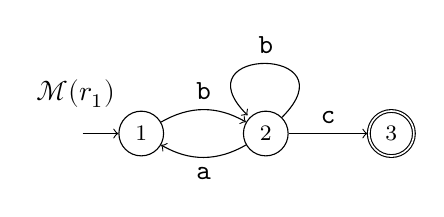
\begin{tikzpicture}
    \tikzset{
      node distance=1cm,
      every state/.append style={minimum size=0.5cm},
      initial text=$ $
    }

    \node[state, initial, label=above left:$\Automaton{r_1}$] (s0) {1};
    \node[state, right=of s0] (s1) {2};
    \node[state, accepting, right=of s1] (s2) {3};

    \draw (s0) edge[->, bend left] node[auto]{$\Char{b}$} (s1);
    \draw (s1) edge[->, bend left] node[auto]{$\Char{a}$} (s0);
    \draw (s1) edge[->, loop] node[above]{$\Char{b}$} (s1);
    \draw (s1) edge[->] node[auto]{$\Char{c}$} (s2);
  \end{tikzpicture}
\end{center}

\Ex

Vsak regularni izraz lahko ustreza večim različnim avtomatom.

\begin{gather*}
  r_2 = \Kleene{(\Char{b} \Seq (\Char{a} \Seq \Char{b})?)} \Seq \Char{c} \\
  \Automaton{r_2} = (Q_2, \Sigma, \delta_2, q_{0, 2}, F_2)
\end{gather*}

\begin{center}
  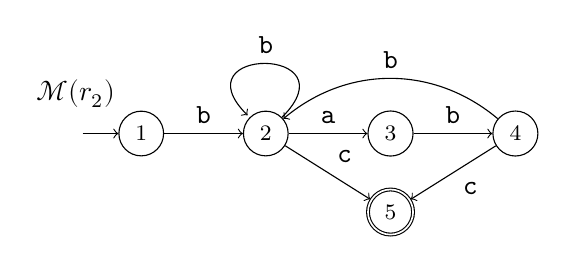
\begin{tikzpicture}
    \tikzset{
      node distance=1cm,
      every state/.append style={minimum size=0.5cm},
      initial text=$ $
    }

    \node[state, initial, label=above left:$\Automaton{r_2}$] (s0) {1};
    \node[state, right=of s0] (s1) {2};
    \node[state, right=of s1] (s2) {3};
    \node[state, right=of s2] (s3) {4};
    \node[state, accepting, below=0.4cm of s2] (s4) {5};

    \draw (s0) edge[->] node[auto]{$\Char{b}$} (s1);
    \draw (s1) edge[->, loop] node[above]{$\Char{b}$} (s1);
    \draw (s1) edge[->] node[auto]{$\Char{a}$} (s2);
    \draw (s2) edge[->] node[auto]{$\Char{b}$} (s3);
    \draw (s1) edge[->] node[auto]{$\Char{c}$} (s4);
    \draw (s3) edge[->] node[auto]{$\Char{c}$} (s4);
    \draw (s3) edge[->, bend right=40] node[above]{$\Char{b}$} (s1);
  \end{tikzpicture}
\end{center}

Funkcijo prehodov lahko definiramo tudi za niz:
\begin{align*} % XXX define empty string
  \Kleene{\delta}(q, \varepsilon) &= q\\
  \Kleene{\delta}(q, a \Seq w) &= \Kleene{\delta}(q', w) \text{, kjer } q' = \delta(q, a) \text{ in } q' \neq \Err
\end{align*}

\Ex
\begin{align*}
  \Kleene{\delta_1}(1, \Str{b}) &= 2 \\
  \Kleene{\delta_1}(1, \Str{ba}) &= 1 \\
  \Kleene{\delta_1}(1, \Str{bab}) &= 2 \\
  \Kleene{\delta_1}(1, \Str{bc}) &= 3 \\
  \Kleene{\delta_1}(1, \Str{babbc}) &= 3 \\
  \Kleene{\delta_1}(2, \Str{bbb}) &= 2 \\
  \Kleene{\delta_1}(2, \Str{abbc}) &= 3
\end{align*}

Jezik, ki ga avtomat opisuje:
\begin{equation*}
  L = \{w \in \Kleene{\Sigma} \mid \Kleene{\delta}(q_0, w) \in F\}
\end{equation*}

\Ex

\begin{align*}
  \Kleene{\delta_1}(1, \Str{bc}) &= 3 \\
  \Kleene{\delta_1}(1, \Str{bbc}) &= 3 \\
  \Kleene{\delta_1}(1, \Str{bbbc}) &= 3 \\
  \cdots \\
  \Kleene{\delta_1}(1, \Str{babc}) &= 3 \\
  \Kleene{\delta_1}(1, \Str{bababc}) &= 3 \\
  \ldots \\
  \Kleene{\delta_1}(1, \Str{babbc}) &= 3 \\
  \Kleene{\delta_1}(1, \Str{babbbc}) &= 3 \\
  \cdots \\
  \Kleene{\delta_1}(1, \Str{bababbc}) &= 3 \\
  \Kleene{\delta_1}(1, \Str{bababbbc}) &= 3 \\
  \cdots \\
\end{align*}

\begin{multline*}
  L = \{ \Str{bc}, \Str{bbc}, \Str{bbbc}, \ldots, \Str{babc}, \Str{bababc}, \ldots,\\
  \Str{babbc},  \Str{babbbc}, \ldots, \Str{bababbc}, \Str{bababbbc}, \dots \}
\end{multline*}

Za implementacijo pregledovalnika je potrebno končnemu avtomatu dodati funkcijo, ki končna stanja preslika v terminale:
\begin{equation*}
  \acc: Q \rightarrow T
\end{equation*}

\section{Konstrukcija}

\Special{Meta:} Jezik regularnega izraza $r$ bo označen kot $\Language{r}$.\\

Regularni izraz v končni avtomat pretvorimo tako, da najprej ustvarimo končne avtomate za posamezne elemente $\Char{a}$, $\Empty$, $\Null$, ki jih nato s pomočjo pravil za konstrukcijo združujemo.

%Pri opisani konstrukciji so vsi prehodi, ki vodijo v katero koli stanje stanje označeni z enakim znakom.
%\begin{center}
%  \begin{tikzpicture}
%    \tikzset{
%      ->,
%      node distance=1cm,
%      every state/.append style={minimum size=0.5cm},
%      initial text=$ $
%    }
%
%
%    \node[state] (s) {};
%
%    \node[left=1 of s] (i1) {$\ldots$};
%    \node[above left=1 of s] (i2) {$\ddots$};
%    \node[below left=1 of s] (i3) {\reflectbox{$\ddots$}};
%    \draw(i1) edge node[auto]{\Char{a}} (s);
%    \draw(i2) edge node[auto]{\Char{a}} (s);
%    \draw(i3) edge node[auto]{\Char{a}} (s);
%
%  \end{tikzpicture}
%\end{center}
%To je posebna lastnost končnih avtomat ustvarjenih s to konstrukcijo in ne velja za poljuben končni avtomat.

Sledijo definicije in pravila za konstrucijo za vse operacije in elemente.

\subsection{Prazen jezik}
\begin{tcolorbox}[title={Definicija}]
\begin{equation*}
  \begin{aligned}
    r &= \Empty\\
    \Language{r} &= \{\}
  \end{aligned}
\end{equation*}
\end{tcolorbox}

\begin{center}
  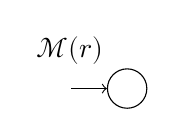
\begin{tikzpicture}
    \tikzset{
      ->,
      node distance=1cm,
      every state/.append style={minimum size=0.5cm},
      initial text=$ $
    }

    \node[state, initial, label=above left:$\Automaton{r}$] {};
  \end{tikzpicture}
\end{center}


\subsection{Prazen niz}

\begin{tcolorbox}[title={Definicija}]
\begin{equation*}
  \begin{aligned}
    r &= \Null\\
    \Language{r} &= \{ \Str{} \}
  \end{aligned}
\end{equation*}
\end{tcolorbox}

\begin{center}
  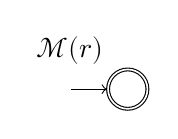
\begin{tikzpicture}
    \tikzset{
      ->,
      node distance=1cm,
      every state/.append style={minimum size=0.5cm},
      initial text=$ $
    }

    \node[state, initial, accepting, label=above left:$\Automaton{r}$] {};
  \end{tikzpicture}
\end{center}

Če $\Str{} \in \Language{r}$, potem rečemo, da je $r$ \emph{nullable}.

\subsection{Znak}

\begin{tcolorbox}[title={Definicija}]
\begin{equation*}
  \begin{aligned}
    r &= \Char{a}\text{, kjer } \Char{a} \in \Alphabet\\\
    \Language{r} &= \{ \Str{a} \}
  \end{aligned}
\end{equation*}
\end{tcolorbox}

\begin{center}
  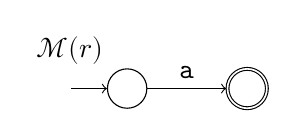
\begin{tikzpicture}
    \tikzset{
      ->,
      node distance=1cm,
      every state/.append style={minimum size=0.5cm},
      initial text=$ $
    }

    \node[state, initial, label=above left:$\Automaton{r}$] (q0) {};
    \node[state, accepting, right=of q0] (q1) {};

    \draw (q0) edge node[auto]{$\Char{a}$} (q1);
  \end{tikzpicture}
\end{center}

\subsection{Množica znakov}
\Reset

\begin{tcolorbox}[title={Definicija}]
\begin{equation*}
  \begin{aligned}
    r &= S\text{, kjer } S \subseteq \Alphabet \\
    &= \Char{a} \Union \dots \Union \Char{b}\text{, kjer } \Char{a}, \dots, \Char{b} \in S\\
    \Language{r} &= S
  \end{aligned}
\end{equation*}
\end{tcolorbox}

\Ex
\begin{equation*}
  \begin{aligned}
    \N{r} &= \{ \Char{a}, \Char{b}, \Char{c} \} \\
    \N{r} &= \Char{a} \Union \Char{b} \Union \Char{c}
  \end{aligned}
\end{equation*}

Množica znakov se lahko predstavi kot šop robov (eden za vsak znak) ali pa en sam rob označen z množico.
\begin{center}
  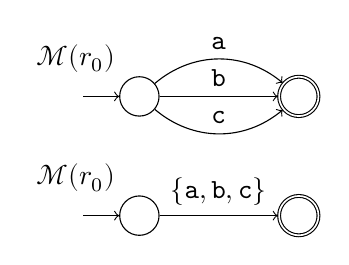
\begin{tikzpicture}
    \tikzset{
      ->,
      node distance=1cm,
      every state/.append style={minimum size=0.5cm},
      initial text=$ $
    }

    \node[state, initial, label=above left:$\Automaton{\N{r}}$] (p0) {};
    \node[state, accepting, right=1.5cm of p0] (p1) {};

    \node[state, initial, below=of p0, label=above left:$\Automaton{\N{r}}$] (q0) {};
    \node[state, accepting, right=1.5cm of q0] (q1) {};


    \draw (q0) edge node[auto]{$\{\Char{a}, \Char{b}, \Char{c} \} $} (q1);

    \draw (p0) edge[bend left=40] node[auto]{$\Char{a}$} (p1);
    \draw (p0) edge node[auto]{$\Char{b}$} (p1);
    \draw (p0) edge[bend right=40] node[auto]{$\Char{c}$} (p1);
  \end{tikzpicture}
\end{center}
\Next

\subsection*{Primeri}

\subsubsection{Y/N}

\begin{equation*}
  \Language{\N{r}} = \{ \Str{Y}, \Str{N} \}
\end{equation*}

\begin{equation*}
  \N{r} = \{ \Char{Y}, \Char{N} \}
\end{equation*}

\begin{center}
  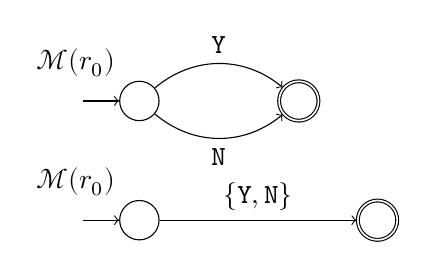
\begin{tikzpicture}
    \tikzset{
      ->,
      node distance=1cm,
      every state/.append style={minimum size=0.5cm},
      initial text=$ $
    }

    \node[state, initial, label=above left:$\Automaton{\N{r}}$] (p0) {};
    \node[state, accepting, right=1.5cm of p0] (p1) {};

    \node[state, initial, below=of p0, label=above left:$\Automaton{\N{r}}$] (q0) {};
    \node[state, accepting, right=2.5cm of q0] (q1) {};


    \draw (q0) edge node[auto]{$\{\Char{Y}, \Char{N} \} $} (q1);

    \draw (p0) edge[bend left=40] node[auto]{$\Char{Y}$} (p1);
    \draw (p0) edge[bend right=40] node[below]{$\Char{N}$} (p1);
  \end{tikzpicture}
\end{center}
\Next

\subsubsection{Števke}

\begin{equation*}
  \Language{\N{r}} = \{ \Str{0}, \Str{1}, \Str{2}, \dots, \Str{9} \}
\end{equation*}

\begin{equation*}
  \N{r} = \{ \Char{0}, \Char{1}, \Char{2}, \dots, \Char{9} \}
\end{equation*}

\begin{center}
  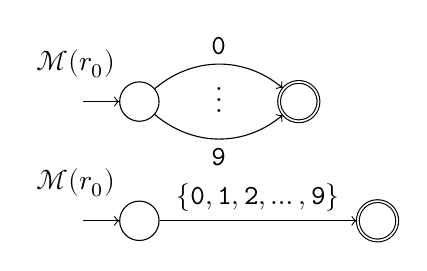
\begin{tikzpicture}
    \tikzset{
      ->,
      node distance=1cm,
      every state/.append style={minimum size=0.5cm},
      initial text=$ $
    }

    \node[state, initial, label=above left:$\Automaton{\N{r}}$] (p0) {};
    \node[state, accepting, right=1.5cm of p0] (p1) {};
    \node at ($(p0)!0.5!(p1)$) {\Dots{}};

    \node[state, initial, below=of p0, label=above left:$\Automaton{\N{r}}$] (q0) {};
    \node[state, accepting, right=2.5cm of q0] (q1) {};


    \draw (q0) edge node[auto]{$\{\Char{0}, \Char{1}, \Char{2}, \ldots, \Char{9} \} $} (q1);

    \draw (p0) edge[bend left=40] node[auto]{$\Char{0}$} (p1);
    \draw (p0) edge[bend right=40] node[below]{$\Char{9}$} (p1);
  \end{tikzpicture}
\end{center}
\Next

\subsubsection{Male črke}

\begin{equation*}
  \Language{\N{r}} = \{ \Str{a}, \Str{b}, \Str{c}, \dots, \Str{z} \}
\end{equation*}
\Next

\subsubsection{Velike in male črke}

\begin{equation*}
  \Language{\N{r}} = \{ \Str{A}, \Str{B}, \Str{C}, \dots, \Str{Z}, \Str{a}, \Str{b}, \Str{c}, \dots, \Str{z} \}
\end{equation*}
\Next

\subsubsection{Heksadecimalne števke}

\begin{equation*}
  \Language{\N{r}} = \{ \Str{0}, \Str{1}, \Str{2}, \dots, \Str{9}, \Str{A}, \dots, \Str{F} \}
\end{equation*}
\Next

\newpage
\subsection{Konkatenacija}
\Reset

\begin{tcolorbox}[title={Definicija}]
\begin{equation*}
  \begin{aligned}
  r &= s \Seq t = s \Spc t\\
  \Language{r} &= \{ u \Seq v \mid u \in \Language{s} \land v \in \Language{t}\}
  \end{aligned}
\end{equation*}
\end{tcolorbox}

\begin{tcolorbox}[title={Pravila}]
\begin{equation*}
  \begin{aligned}
  s \Seq t &\not= t \Seq s\\
  s \Seq \Null &= s \\
  \Null \Seq s &= s   \\
  s \Seq \Empty &= \Empty \\
  \Empty \Seq s &= \Empty \\
  (s \Seq p) \Seq q &= s \Seq (p \Seq q) = s \Seq p \Seq q
  \end{aligned}
\end{equation*}
\end{tcolorbox}

\vspace{1em}
\Special{Poseben primer:} Če $|\Language{s}| = |\Language{t}| = 1$, potem $\Language{s} = \{u\}$ in $\Language{t} = \{v\}$ in $\Language{r} = \{u \Seq v\}$.

\Ex
\begin{align*}
  \Language{s} &= \{\Str{Hello}\}\\
  \Language{t} &= \{\Str{World}\}\\
  \Language{r} &= \{\Str{HelloWorld}\}
\end{align*}

Splošno je jezik konkatenacije podoben kartezičnemu produktu.
\begin{align*}
  S &= P \times Q \\
  S &= \{ (x, y) \mid x \in P \land y \in Q\}
\end{align*}

\Ex
\begin{align*}
  P &= \{1, 2, 3\}\\
  Q &= \{a, b\}\\
  S &= \{(1, a), (1, b), (2, a), (2, b), (3, a), (3, b) \}
\end{align*}

Edina razlika je da zamenjamo vsak $(u, v)$, kjer $u \in \Language{s}$ in $v\in \Language{t}$, z $u \Seq v \in \Language{r}$.

\Ex

\begin{align*}
  P &= \{\Str{Dober}, \Str{Lep}\}\\
  Q &= \{\Str{Dan}, \Str{Večer}, \Str{Tek}\}\\
  S &= \{\Str{DoberDan}, \Str{DoberVečer}, \Str{DoberTek}, \Str{LepDan}, \Str{LepVečer}, \Str{LepTek} \}
\end{align*}

Končni avtomat konkatenacije $\Automaton{r}$ dveh končnih avtomatov $\Automaton{s}$ in $\Automaton{t}$ sestavimo tako:
\begin{enumerate}
  \item Ustvarimo prehod $\delta(q, \Char{a}) = q'$ iz vsakega končnega stanja $q$ v $\Automaton{s}$ v vsako stanje $q'$, ki je direktno dosegljivo iz začetnega stanja v $\Automaton{t}$ (vsakega z vsakim). 
    Ustvarjen prehod je označen z enakim simbolom $\Char{a}$, kot obstoječi prehod, ki vodi iz začetnega stanja v $q'$.
  \item Začetno stanje $\Automaton{t}$ odstranimo.
  \item Končna stanja $\Automaton{s}$ označimo kot ne-končna, razen če je končno začetno stanje $\Automaton{t}$.
\end{enumerate}

\begin{center}
  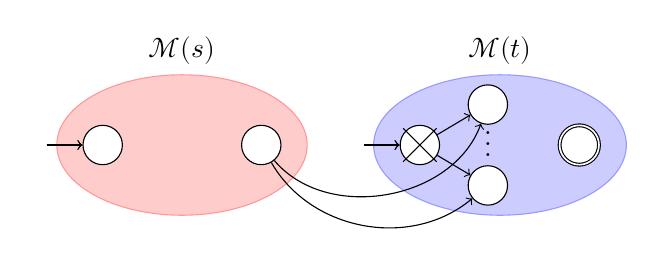
\begin{tikzpicture}
    \tikzset{
      node distance=1cm,
      every state/.append style={fill=white, minimum size=0.5cm},
      initial text=$ $
    }

    \node[initial, state, initial] (s0) {};
    \node[state, hide, above right=0.15cm and 0.5cm of s0] (s1) {};
    \node[state, hide, fill=none, below right=0.15cm and 0.5cm of s0] (s2) {};
    \node[state, right=1.5cm of s0] (sn) {};

    \begin{pgfonlayer}{background}
      \node[fit=(s0) (s1) (s2) (sn), draw=red!40, fill=red!20, ellip, label=above:$\Automaton{s}$] (qm) {};
    \end{pgfonlayer}

    \node[initial, state, initial, right=1.5cm of sn] (p0) {};
    \path (p0) pic {cross=0.30cm};
    \node[state, above right=0.15cm and 0.5cm of p0] (p1) {};
    \node[state, below right=0.15cm and 0.5cm of p0] (p2) {};
    \node at ($(p1)!0.5!(p2)$) {\Dots{}};
    \draw (p0) edge[->] (p1);
    \draw (p0) edge[->] (p2);
    \draw (sn) edge[->, bend right=60] (p1);
    \draw (sn) edge[->, bend right=50] (p2);
    \node[state, accepting, right=1.5cm of p0] (pn) {};

    \begin{pgfonlayer}{background}
      \node[fit=(p0) (p1) (p2) (pn), ellip, draw=blue!40, fill=blue!20, label=above:$\Automaton{t}$] (pm) {};
    \end{pgfonlayer}
  \end{tikzpicture}
\end{center}

\Ex
\begin{align*}
  \N{s} &= \Char{a} \\
  \N{t} &= \Char{b} \\
  \N{r} &= \Char{a} \Spc \Char{b} \\
\end{align*}

\begin{align*}
  \Language{\N{s}} &= \{\Str{a}\} \\
  \Language{\N{t}} &= \{\Str{b}\} \\
  \Language{\N{r}} &= \{\Str{ab}\}
\end{align*}

\begin{center}
  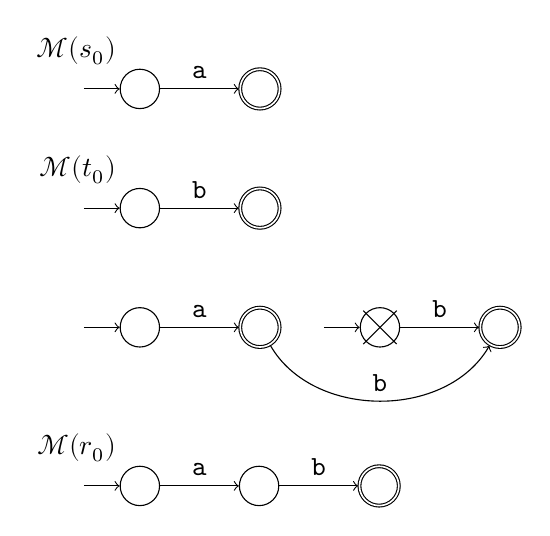
\begin{tikzpicture}
    \tikzset{
      node distance=1cm,
      every state/.append style={minimum size=0.5cm},
      initial text=$ $
    }

    \node[state, initial, label=above left:$\Automaton{\N{s}}$] (x0) {};
    \node[state, accepting, right=of x0] (x1) {};

    \draw (x0) edge[->] node[auto]{$\Char{a}$} (x1);

    \node[state, initial, label=above left:$\Automaton{\N{t}}$, below=of x0] (y0) {};
    \node[state, accepting, right=of y0] (y1) {};

    \draw (y0) edge[->] node[auto]{$\Char{b}$} (y1);

    \node[state, initial, below=of y0] (q0) {};
    \node[state, accepting, right=of q0] (q1) {};

    \draw (q0) edge[->] node[auto]{$\Char{a}$} (q1);

    \node[state, initial, right=of q1] (p0) {};
    \path (p0) pic {cross=0.30cm};
    \node[state, accepting, right=of p0] (p1) {};

    \draw (p0) edge[->] node[auto]{$\Char{b}$} (p1);

    \draw (q1) edge[->, bend right=60] node[auto]{$\Char{b}$} (p1);

    \node[state, initial, label=above left:$\Automaton{\N{r}}$, below=1.5cm of q0] (s0) {};
    \node[state, right=of s0] (s1) {};
    \node[state, accepting, right=of s1] (s2) {};

    \draw (s0) edge[->] node[auto]{$\Char{a}$} (s1);
    \draw (s1) edge[->] node[auto]{$\Char{b}$} (s2);
  \end{tikzpicture}
\end{center}
\Next

\Ex

\begin{align*}
  \N{s} &= \Char{a} \Spc \Char{b} \\
  \N{t} &= \Char{c} \\
  \N{r} &= \Char{a} \Spc \Char{b} \Spc \Char{c} \\
\end{align*}

\begin{align*}
  \Language{\N{s}} &= \{\Str{ab}\} \\
  \Language{\N{t}} &= \{\Str{c}\} \\
  \Language{\N{r}} &= \{\Str{abc}\}
\end{align*}

\begin{center}
  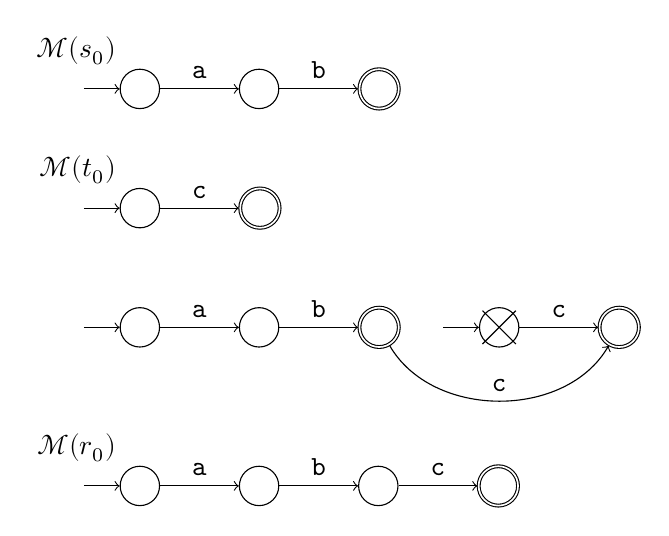
\begin{tikzpicture}
    \tikzset{
      node distance=1cm,
      every state/.append style={minimum size=0.5cm},
      initial text=$ $
    }

    \node[state, initial, label=above left:$\Automaton{\N{s}}$] (x0) {};
    \node[state, right=of x0] (x1) {};
    \node[state, accepting, right=of x1] (x2) {};

    \draw (x0) edge[->] node[auto]{$\Char{a}$} (x1);
    \draw (x1) edge[->] node[auto]{$\Char{b}$} (x2);

    \node[state, initial, label=above left:$\Automaton{\N{t}}$, below=of x0] (y0) {};
    \node[state, accepting, right=of y0] (y1) {};

    \draw (y0) edge[->] node[auto]{$\Char{c}$} (y1);

    \node[state, initial, below=of y0] (q0) {};
    \node[state, right=of q0] (q1) {};
    \node[state, accepting, right=of q1] (q2) {};

    \draw (q0) edge[->] node[auto]{$\Char{a}$} (q1);
    \draw (q1) edge[->] node[auto]{$\Char{b}$} (q2);

    \node[state, initial, right=of q2] (p0) {};
    \path (p0) pic {cross=0.30cm};
    \node[state, accepting, right=of p0] (p1) {};

    \draw (p0) edge[->] node[auto]{$\Char{c}$} (p1);

    \draw (q2) edge[->, bend right=60] node[auto]{$\Char{c}$} (p1);

    \node[state, initial, label=above left:$\Automaton{\N{r}}$, below=1.5cm of q0] (s0) {};
    \node[state, right=of s0] (s1) {};
    \node[state, right=of s1] (s2) {};
    \node[state, accepting, right=of s2] (s3) {};

    \draw (s0) edge[->] node[auto]{$\Char{a}$} (s1);
    \draw (s1) edge[->] node[auto]{$\Char{b}$} (s2);
    \draw (s2) edge[->] node[auto]{$\Char{c}$} (s3);
  \end{tikzpicture}
\end{center}
\Next

\Ex
\begin{align*}
  \N{s} &= \Char{a} \Spc \Char{b} \\
  \N{t} &= \Char{c} \Spc \Char{d} \\
  \N{r} &= \Char{a} \Spc \Char{b} \Spc \Char{c} \Spc \Char{d} \\
\end{align*}

\begin{align*}
  \Language{\N{s}} &= \{\Str{ab}\} \\
  \Language{\N{t}} &= \{\Str{cd}\} \\
  \Language{\N{r}} &= \{\Str{abcd}\}
\end{align*}

\begin{center}
  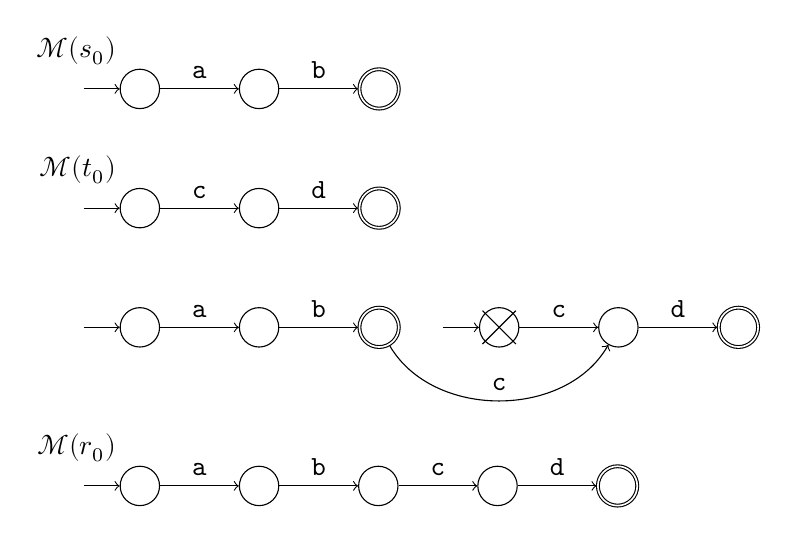
\begin{tikzpicture}
    \tikzset{
      node distance=1cm,
      every state/.append style={minimum size=0.5cm},
      initial text=$ $
    }

    \node[state, initial, label=above left:$\Automaton{\N{s}}$] (x0) {};
    \node[state, right=of x0] (x1) {};
    \node[state, accepting, right=of x1] (x2) {};

    \draw (x0) edge[->] node[auto]{$\Char{a}$} (x1);
    \draw (x1) edge[->] node[auto]{$\Char{b}$} (x2);

    \node[state, initial, label=above left:$\Automaton{\N{t}}$, below=of x0] (y0) {};
    \node[state, right=of y0] (y1) {};
    \node[state, accepting, right=of y1] (y2) {};

    \draw (y0) edge[->] node[auto]{$\Char{c}$} (y1);
    \draw (y1) edge[->] node[auto]{$\Char{d}$} (y2);

    \node[state, initial, below=of y0] (q0) {};
    \node[state, right=of q0] (q1) {};
    \node[state, accepting, right=of q1] (q2) {};

    \draw (q0) edge[->] node[auto]{$\Char{a}$} (q1);
    \draw (q1) edge[->] node[auto]{$\Char{b}$} (q2);

    \node[state, initial, right=of q2] (p0) {};
    \path (p0) pic {cross=0.30cm};
    \node[state, right=of p0] (p1) {};
    \node[state, accepting, right=of p1] (p2) {};

    \draw (p0) edge[->] node[auto]{$\Char{c}$} (p1);
    \draw (p1) edge[->] node[auto]{$\Char{d}$} (p2);

    \draw (q2) edge[->, bend right=60] node[auto]{$\Char{c}$} (p1);

    \node[state, initial, label=above left:$\Automaton{\N{r}}$, below=1.5cm of q0] (s0) {};
    \node[state, right=of s0] (s1) {};
    \node[state, right=of s1] (s2) {};
    \node[state, right=of s2] (s3) {};
    \node[state, accepting, right=of s3] (s4) {};

    \draw (s0) edge[->] node[auto]{$\Char{a}$} (s1);
    \draw (s1) edge[->] node[auto]{$\Char{b}$} (s2);
    \draw (s2) edge[->] node[auto]{$\Char{c}$} (s3);
    \draw (s3) edge[->] node[auto]{$\Char{d}$} (s4);
  \end{tikzpicture}
\end{center}
\Next

\subsection*{Primeri}

\subsubsection{"then"}
\begin{equation*}
  \Language{\N{r}} = \{ \Str{then} \}
\end{equation*}
\Next

\subsubsection{"then", "Then", "THEN", "theN", ...}
Če so robovi avtomatov označeni z množico znakov, avtomat konkatenacije sestavimo na čisto enak način, kot če bi bil na robovih en sam znak.
\begin{equation*}
  \N{r} = \{\Char{T}, \Char{t}\} \Seq \{\Char{H}, \Char{h}\} \Seq \{\Char{E}, \Char{e}\} \Seq \{\Char{N}, \Char{n}\}
\end{equation*}

\Next
\subsubsection{Bajt po osmiško}

\begin{equation*}
  \N{r} = \{\Char{0}, \dots, \Char{3}\} \Seq \{\Char{0}, \dots, \Char{7}\} \Seq \{\Char{0}, \dots, \Char{7}\}
\end{equation*}

\begin{equation*}
  \Language{\N{r}} = \{ \Str{000}, \Str{001}, \Str{002}, \dots, \Str{377} \}
\end{equation*}
\Next

\subsection{Potence}
\Reset

\begin{tcolorbox}[title={Definicija}]
\begin{equation*}
  \begin{aligned}
    \Rep{s}{0} &= \Null\\
    \Rep{s}{i+1} &= \Rep{s}{i} \Seq s\\[1em]
    \Rep{s}{i} &= \underbrace{s \Seq \ldots \Seq s}_{i}\\[1em]
    \Language{\Rep{s}{0}} &= \Null\\
    \Language{\Rep{s}{i+1}} &= \{u \Seq v \mid u \in \Language{\Rep{s}{i}} \land v \in \Language{s}\}
  \end{aligned}
\end{equation*}
\end{tcolorbox}
\begin{align*}
\end{align*}

Avtomat $\Automaton{\Rep{s}{i}}$ sestavimo tako, da konkateniramo $i$ kopij avtomata $\Automaton{s}$.
Avtomat $\Automaton{\Rep{s}{0}}$ je enak, kot avtomat za prazen niz.

\begin{center}
  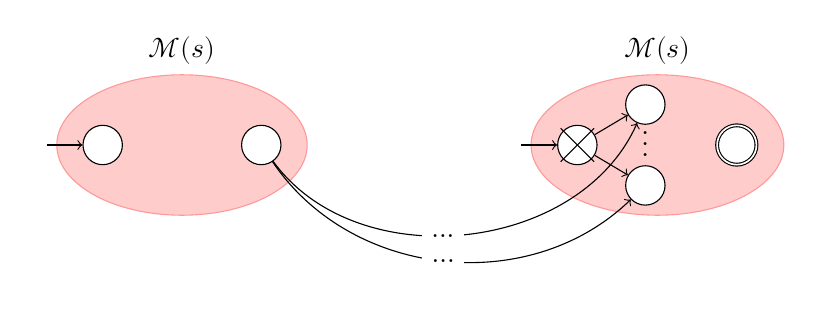
\begin{tikzpicture}
    \tikzset{
      node distance=1cm,
      every state/.append style={fill=white, minimum size=0.5cm},
      initial text=$ $
    }

    \node[state, initial] (s0) {};
    \node[state, hide, above right=0.15cm and 0.5cm of s0] (s1) {};
    \node[state, hide, below right=0.15cm and 0.5cm of s0] (s2) {};
    \node[state, right=1.5cm of s0] (sn) {};

    \begin{pgfonlayer}{background}
      \node[fit=(s0) (s1) (s2) (sn), ellip, draw=red!40, fill=red!20, label=above:$\Automaton{s}$] (qm) {};
    \end{pgfonlayer}

    \node[state, initial, right=3.5cm of sn] (p0) {};
    \path (p0) pic {cross=0.30cm};
    \node[state, above right=0.15cm and 0.5cm of p0] (p1) {};
    \node[state, below right=0.15cm and 0.5cm of p0] (p2) {};
    \node at ($(p1)!0.5!(p2)$) {\Dots{}};
    \draw (p0) edge[->] (p1);
    \draw (p0) edge[->] (p2);
    \draw (sn) edge[->, bend right=60] node[pos=0.45,fill=white] {...} (p1);
    \draw (sn) edge[->, bend right=50] node[pos=0.5,fill=white] {...} (p2);
    \node[state, accepting, right=1.5cm of p0] (pn) {};

    \begin{pgfonlayer}{background}
      \node[fit=(p0) (p1) (p2) (pn), ellip, draw=red!40, fill=red!20, label=above:$\Automaton{s}$] (pm) {};
    \end{pgfonlayer}
  \end{tikzpicture}
\end{center}

\subsection*{Primeri}

\subsubsection{"aaaa"}

\begin{align*}
  \N{s} &= \Char{a} \\
  \N{r} &= \Char{a}^4
\end{align*}

\begin{align*}
  \Language{\N{s}} &= \{\Str{a}\} \\
  \Language{\N{r}} &= \{\Str{aaaa}\} \\
\end{align*}
\Next

\subsubsection{"abab"}

\begin{align*}
  \N{s} &= \Char{a} \Spc \Char{b} \\
  \N{r} &= (\Char{a} \Spc \Char{b})^2
\end{align*}

\begin{align*}
  \Language{\N{s}} &= \{\Str{ab}\} \\
  \Language{\N{r}} &= \{\Str{abab}\} \\
\end{align*}
\Next

\subsubsection{Bajt po osmiško}
\begin{equation*}
  \N{r} = \{\Char{0}, \dots, \Char{3}\} \Seq (\{\Char{0}, \dots, \Char{7}\})^2
\end{equation*}
\Next

\subsection{Unija}
\Reset

\begin{tcolorbox}[title={Definicija}]
  \begin{equation*}
    \begin{aligned}
    r &= s \Union t \\
      \Language{r} &= \Language{s} \cup \Language{t}
    \end{aligned}
  \end{equation*}
\end{tcolorbox}

\begin{tcolorbox}[title={Pravila}]
  \begin{equation*}
    \begin{aligned}
      s \Union t &= t \Union s \\
      s \Union s &= s \\
      \Empty \Union s &= s \\
      s \Union \Empty &= s \\
      (s \Union p) \Union q &= s \Union (p \Union q) = s \Union p \Union q \\
      s \Seq (p \Union q) &= s \Seq p \Union s \Seq q\\
      (p \Union q) \Seq s &= p \Seq s \Union q \Seq s\\
    \end{aligned}
  \end{equation*}
\end{tcolorbox}

Končni avtomat unije $\Automaton{r}$ dveh končnih avtomatov $\Automaton{s}$ in $\Automaton{t}$ sestavimo tako:
\begin{enumerate}
\item Ustvarimo novo začetno stanje $q$.

\item Ustvarimo prehod $\delta(q, \Char{a}) = q'$ iz novega začetnega stanja $q$ v vsako stanje $q'$, ki je direktno dosegljivo iz začetnega stanja v $\Automaton{s}$ ali $\Automaton{t}$.
    Ustvarjen prehod je označen z enakim simbolom $\Char{a}$, kot obstoječi prehod, ki vodi iz začetnega stanja v $q'$.
\item Začetni stanji $\Automaton{s}$ in $\Automaton{t}$ odstranimo.
\item Začetno stanje $\Automaton{r}$ je končno če je končno začetno stanje $\Automaton{s}$ ali $\Automaton{t}$.
\end{enumerate}

\begin{center}
  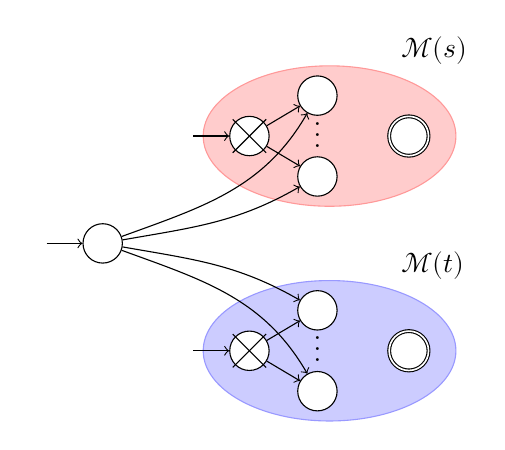
\begin{tikzpicture}
    \tikzset{
      node distance=1cm,
      every state/.append style={fill=white, minimum size=0.5cm},
      initial text=$ $
    }

    \node[state, initial] (q0) {};

    \node[state, above right=1.0cm and 1.5cm of q0, initial] (s0) {};
    \path (s0) pic {cross=0.30cm};
    \node[state, above right=0.15cm and 0.5cm of s0] (s1) {};
    \node[state, below right=0.15cm and 0.5cm of s0] (s2) {};
    \node at ($(s1)!0.5!(s2)$) {\Dots{}};
    \draw (s0) edge[->] (s1);
    \draw (s0) edge[->] (s2);
    \draw (q0) edge[->, out=20+0, in=-120] (s1);
    \draw (q0) edge[->, out=10+0, in=-150+0] (s2);
    \node[state, accepting, right=1.5cm of s0] (sn) {};

    \begin{pgfonlayer}{background}
      \node[fit=(s0) (s1) (s2) (sn), ellip, draw=red!40, fill=red!20, label=above right:$\Automaton{s}$] (qm) {};
    \end{pgfonlayer}

    \node[state, below right=1.0cm and 1.5cm of q0, initial] (p0) {};
    \path (p0) pic {cross=0.30cm};
    \node[state, above right=0.15cm and 0.5cm of p0] (p1) {};
    \node[state, below right=0.15cm and 0.5cm of p0] (p2) {};
    \node at ($(p1)!0.5!(p2)$) {\Dots{}};
    \draw (p0) edge[->] (p1);
    \draw (p0) edge[->] (p2);
    \draw (q0) edge[->, out=-10+0, in=150+0] (p1);
    \draw (q0) edge[->, out=-20+0, in=120] (p2);
    \node[state, accepting, right=1.5cm of p0] (pn) {};

    \begin{pgfonlayer}{background}
      \node[fit=(p0) (p1) (p2) (pn), ellip, draw=blue!40, fill=blue!20, label=above right:$\Automaton{t}$] (pm) {};
    \end{pgfonlayer}
  \end{tikzpicture}
\end{center}

\Ex
\begin{align*}
  \N{s} &= \Char{a} \\
  \N{t} &= \Char{b} \\
  \N{r} &= \Char{a} \Union \Char{b}
\end{align*}

\begin{align*}
  \Language{\N{s}} &= \{\Str{a}\} \\
  \Language{\N{t}} &= \{\Str{b}\} \\
  \Language{\N{r}} &= \{\Str{a}, \Str{b}\} \\
\end{align*}

\begin{center}
  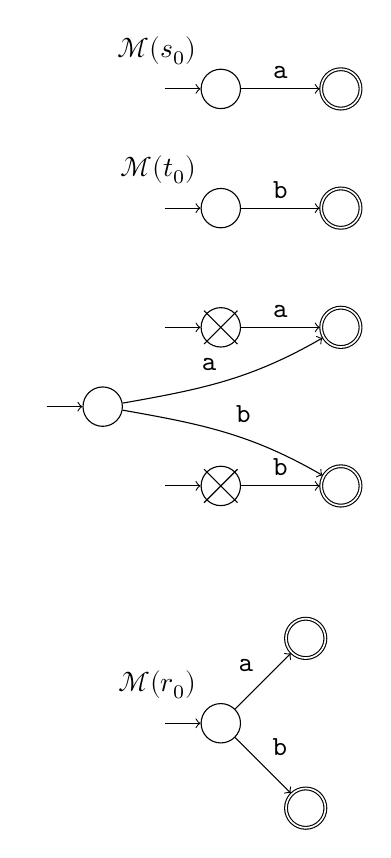
\begin{tikzpicture}
    \tikzset{
      node distance=1cm,
      every state/.append style={minimum size=0.5cm},
      initial text=$ $
    }

    \node[state, initial, label=above left:$\Automaton{\N{s}}$] (x0) {};
    \node[state, accepting, right=of x0] (x1) {};

    \draw (x0) edge[->] node[auto]{$\Char{a}$} (x1);

    \node[state, initial, label=above left:$\Automaton{\N{t}}$, below=of x0] (y0) {};
    \node[state, accepting, right=of y0] (y1) {};

    \draw (y0) edge[->] node[auto]{$\Char{b}$} (y1);

    \node[state, initial, below=of y0] (q0) {};
    \path (q0) pic {cross=0.30cm};
    \node[state, accepting, right=of q0] (q1) {};

    \draw (q0) edge[->] node[auto]{$\Char{a}$} (q1);

    \node[state, initial, below=1.5cm of q0] (p0) {};
    \path (p0) pic {cross=0.30cm};
    \node[state, accepting, right=of p0] (p1) {};

    \draw (p0) edge[->] node[auto]{$\Char{b}$} (p1);

    \node[state, initial] at ($(q0)!0.5!(p0) - (1.5, 0)$) (n) {};

    \draw (n) edge[->, out=10+0, in=-150+0] node[auto] {$\Char{a}$} (q1);
    \draw (n) edge[->, out=-10+0, in=150+0] node[auto] {$\Char{b}$} (p1);

    \node[state, initial, below=2.5cm of p0, label=above left:$\Automaton{\N{r}}$] (u0) {};
    \node[state, accepting, above right=of u0] (u1) {};

    \draw (u0) edge[->] node[auto]{$\Char{a}$} (u1);

    \node[state, accepting, below right=of u0] (u4) {};

    \draw (u0) edge[->] node[auto]{$\Char{b}$} (u4);

  \end{tikzpicture}
\end{center}
\Next

\Ex
\begin{align*}
  \N{s} &= \Char{a} \Union \Char{b} \\
  \N{t} &= \Char{c} \Union \Char{d} \\
  \N{r} &= (\Char{a} \Union \Char{b}) \Seq (\Char{c} \Union \Char{d})
\end{align*}

\begin{align*}
  \Language{\N{s}} &= \{\Str{a}, \Str{b}\} \\
  \Language{\N{t}} &= \{\Str{c}, \Str{d}\} \\
  \Language{\N{r}} &= \{\Str{ac}, \Str{ad}, \Str{bc}, \Str{bd}\} \\
\end{align*}

\begin{center}
  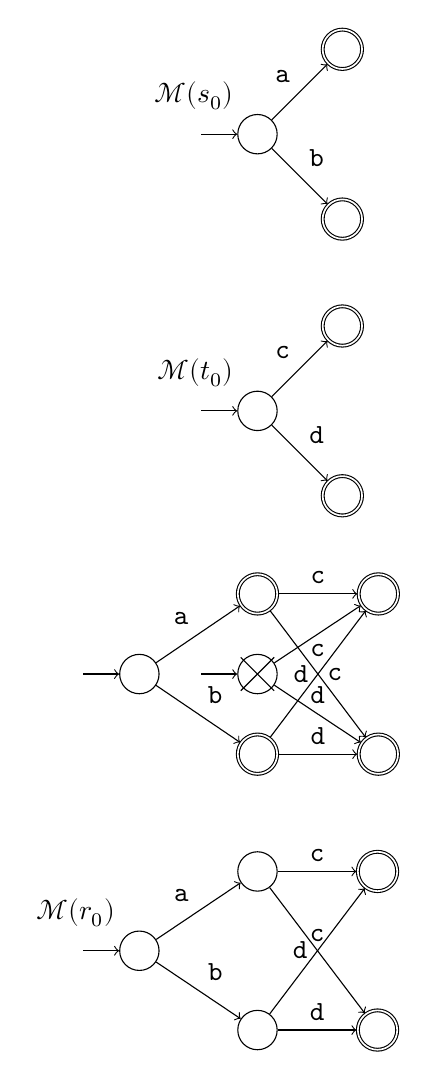
\begin{tikzpicture}
    \tikzset{
      node distance=1cm,
      every state/.append style={minimum size=0.5cm},
      initial text=$ $
    }

    \node[state, initial, label=above left:$\Automaton{\N{s}}$] (x0) {};
    \node[state, accepting, above right=of x0] (x1) {};
    \node[state, accepting, below right=of x0] (x2) {};

    \draw (x0) edge[->] node[auto]{$\Char{a}$} (x1);
    \draw (x0) edge[->] node[auto]{$\Char{b}$} (x2);

    \node[state, initial, label=above left:$\Automaton{\N{t}}$, below=3 of x0] (y0) {};
    \node[state, accepting, above right=of y0] (y1) {};
    \node[state, accepting, below right=of y0] (y2) {};

    \draw (y0) edge[->] node[auto]{$\Char{c}$} (y1);
    \draw (y0) edge[->] node[auto]{$\Char{d}$} (y2);

    \node[state, accepting, below=1.8 of y0] (q0) {};
    \node[state, accepting, right=of q0] (q1) {};

    \draw (q0) edge[->] node[auto]{$\Char{c}$} (q1);

    \node[state, accepting, below=1.5cm of q0] (p0) {};
    \node[state, accepting, right=of p0] (p1) {};

    \draw (p0) edge[->] node[auto]{$\Char{d}$} (p1);

    \node[state, initial] at ($(q0)!0.5!(p0) - (1.5, 0)$) (n) {};

    \node[state, initial] at ($(q0)!0.5!(p0)$) (n1) {};
    \path (n1) pic {cross=0.30cm};

    \draw (n) edge[->] node[auto] {$\Char{a}$} (q0);
    \draw (n) edge[->] node[auto] {$\Char{b}$} (p0);

    \draw (n1) edge[->] node[below] {$\Char{c}$} (q1);
    \draw (n1) edge[->] node[above] {$\Char{d}$} (p1);

    \draw (p0) edge[->] node[right] {$\Char{c}$} (q1);
    \draw (q0) edge[->] node[left] {$\Char{d}$} (p1);

    \node[state, below=3.0 of q0] (e0) {};
    \node[state, accepting, right=of e0] (e1) {};

    \draw (e0) edge[->] node[auto]{$\Char{c}$} (e1);

    \node[state, below=1.5cm of e0] (f0) {};
    \node[state, accepting, right=of f0] (f1) {};

    \draw (f0) edge[->] node[auto]{$\Char{d}$} (f1);

    \node[state, initial, label=above left:$\Automaton{\N{r}}$] at ($(e0)!0.5!(f0) - (1.5, 0)$) (m) {};

    \draw (m) edge[->] node[auto] {$\Char{a}$} (e0);
    \draw (m) edge[->] node[auto] {$\Char{b}$} (f0);

    \draw (f0) edge[->] node[above] {$\Char{c}$} (e1);
    \draw (e0) edge[->] node[left] {$\Char{d}$} (f1);

  \end{tikzpicture}
\end{center}
\Next

\Ex
\begin{align*}
  \N{s} &= \Char{a} \Spc \Char{b} \\
  \N{t} &= \Char{c} \Spc \Char{d} \\
  \N{r} &= \Char{a} \Spc \Char{b} \Union \Char{c} \Spc \Char{d}
\end{align*}

\begin{align*}
  \Language{\N{s}} &= \{\Str{ab}\} \\
  \Language{\N{t}} &= \{\Str{cd}\} \\
  \Language{\N{r}} &= \{\Str{ab}, \Str{cd}\} \\
\end{align*}

\begin{center}
  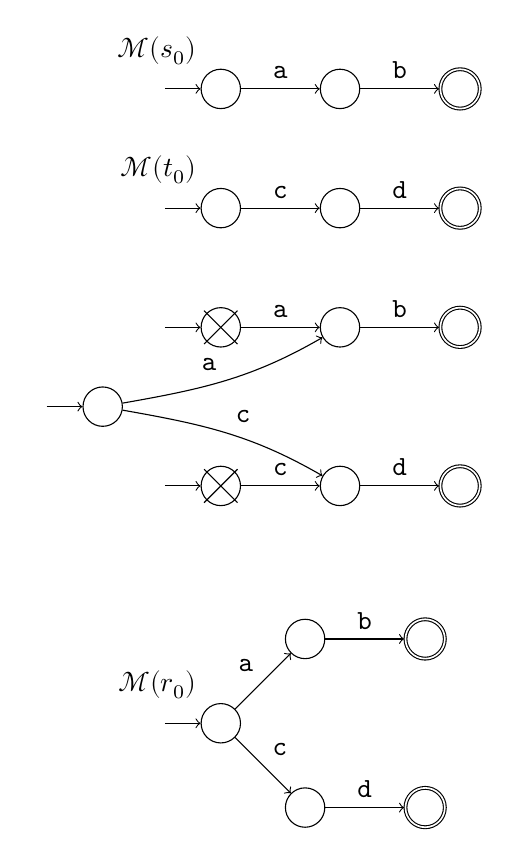
\begin{tikzpicture}
    \tikzset{
      node distance=1cm,
      every state/.append style={minimum size=0.5cm},
      initial text=$ $
    }

    \node[state, initial, label=above left:$\Automaton{\N{s}}$] (x0) {};
    \node[state, right=of x0] (x1) {};
    \node[state, accepting, right=of x1] (x2) {};

    \draw (x0) edge[->] node[auto]{$\Char{a}$} (x1);
    \draw (x1) edge[->] node[auto]{$\Char{b}$} (x2);

    \node[state, initial, label=above left:$\Automaton{\N{t}}$, below=of x0] (y0) {};
    \node[state, right=of y0] (y1) {};
    \node[state, accepting, right=of y1] (y2) {};

    \draw (y0) edge[->] node[auto]{$\Char{c}$} (y1);
    \draw (y1) edge[->] node[auto]{$\Char{d}$} (y2);

    \node[state, initial, below=of y0] (q0) {};
    \path (q0) pic {cross=0.30cm};
    \node[state, right=of q0] (q1) {};
    \node[state, accepting, right=of q1] (q2) {};

    \draw (q0) edge[->] node[auto]{$\Char{a}$} (q1);
    \draw (q1) edge[->] node[auto]{$\Char{b}$} (q2);

    \node[state, initial, below=1.5cm of q0] (p0) {};
    \path (p0) pic {cross=0.30cm};
    \node[state, right=of p0] (p1) {};
    \node[state, accepting, right=of p1] (p2) {};

    \draw (p0) edge[->] node[auto]{$\Char{c}$} (p1);
    \draw (p1) edge[->] node[auto]{$\Char{d}$} (p2);

    \node[state, initial] at ($(q0)!0.5!(p0) - (1.5, 0)$) (n) {};

    \draw (n) edge[->, out=10+0, in=-150+0] node[auto] {$\Char{a}$} (q1);
    \draw (n) edge[->, out=-10+0, in=150+0] node[auto] {$\Char{c}$} (p1);

    \node[state, initial, below=2.5cm of p0, label=above left:$\Automaton{\N{r}}$] (u0) {};
    \node[state, above right=of u0] (u1) {};
    \node[state, accepting, right=of u1] (u2) {};

    \draw (u0) edge[->] node[auto]{$\Char{a}$} (u1);
    \draw (u1) edge[->] node[auto]{$\Char{b}$} (u2);

    \node[state, below right=of u0] (u4) {};
    \node[state, accepting, right=of u4] (u5) {};

    \draw (u0) edge[->] node[auto]{$\Char{c}$} (u4);
    \draw (u4) edge[->] node[auto]{$\Char{d}$} (u5);

  \end{tikzpicture}
\end{center}
\Next

\Special{Poseben primer:} Če nizi v $\Language{s}$ in $\Language{t}$ nimajo skupne predpone bodo znaki na robovih, ki izhajajo iz začetnih stanj $\Automaton{s}$ in $\Automaton{t}$ različni. Nastali končni avtomat bo posledično determinističen.

\Ex

\begin{align*}
  \N{s} &= \Char{a} \Spc \Char{b} \\
  \N{p} &= \Char{a} \Spc \Char{b} \Spc \Char{c} \\
  \N{t} &= \Char{a} \Spc \Char{c} \Spc \Char{d} \\
  \N{r} &= \N{s} \Union \N{p} \Union \N{t} \\
\end{align*}

\begin{center}
  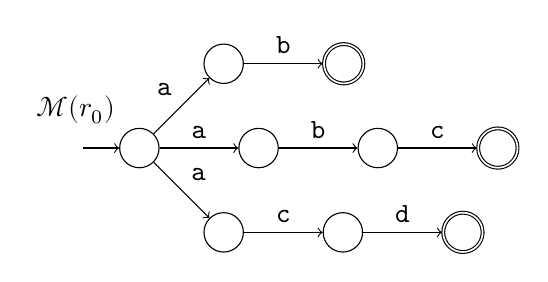
\begin{tikzpicture}
    \tikzset{
      node distance=1cm,
      every state/.append style={minimum size=0.5cm},
      initial text=$ $
    }

    \node[state, initial, label=above left:$\Automaton{\N{r}}$] (u0) {};
    \node[state, right=of u0] (u1) {};
    \node[state, right=of u1] (u2) {};
    \draw (u0) edge[->] node[auto]{$\Char{a}$} (u1);
    \draw (u1) edge[->] node[auto]{$\Char{b}$} (u2);

    \node[state, accepting, right=of u2] (u3) {};
    \draw (u2) edge[->] node[auto]{$\Char{c}$} (u3);

    \node[state, below right=of u0] (u6) {};

    \node[state, right=of u6] (u4) {};
    \node[state, accepting, right=of u4] (u5) {};

    \draw (u0) edge[->] node[auto]{$\Char{a}$} (u6);
    \draw (u6) edge[->] node[auto]{$\Char{c}$} (u4);
    \draw (u4) edge[->] node[auto]{$\Char{d}$} (u5);

    \node[state, above right=of u0] (u7) {};
    \node[state, accepting, right=of u7] (u8) {};

    \draw (u0) edge[->] node[auto]{$\Char{a}$} (u7);
    \draw (u7) edge[->] node[auto]{$\Char{b}$} (u8);

  \end{tikzpicture}
\end{center}

\subsection*{Leva faktorizacija}
Skupno predpono izpostavimo.

\Ex
\begin{align*}
  \N{r} &= \Char{a} \Spc \Char{b} \Union \Char{a} \Spc \Char{b} \Spc \Char{c} \Union \Char{a} \Spc \Char{c} \Spc \Char{d}\\
        &= \Char{a} \Seq (\Char{b} \Union \Char{b} \Spc \Char{c} \Union \Char{c} \Spc \Char{d})\\
        &= \Char{a} \Seq (\Char{b} \Seq (\Null \Union \Char{c}) \Union \Char{c} \Spc \Char{d})
\end{align*}

\begin{center}
  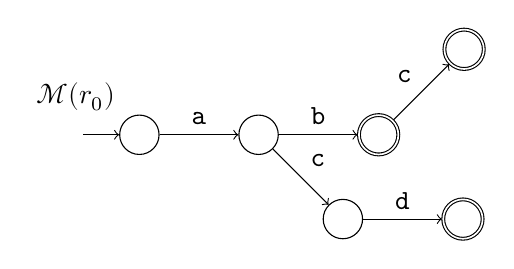
\begin{tikzpicture}
    \tikzset{
      node distance=1cm,
      every state/.append style={minimum size=0.5cm},
      initial text=$ $
    }

    \node[state, initial, label=above left:$\Automaton{\N{r}}$] (u0) {};
    \node[state, right=of u0] (u1) {};
    \node[state, accepting, right=of u1] (u2) {};
    \draw (u0) edge[->] node[auto]{$\Char{a}$} (u1);
    \draw (u1) edge[->] node[auto]{$\Char{b}$} (u2);

    \node[state, accepting, above right=of u2] (u3) {};
    \draw (u2) edge[->] node[auto]{$\Char{c}$} (u3);

    \node[state, below right=of u1] (u4) {};
    \node[state, accepting, right=of u4] (u5) {};

    \draw (u1) edge[->] node[auto]{$\Char{c}$} (u4);
    \draw (u4) edge[->] node[auto]{$\Char{d}$} (u5);

  \end{tikzpicture}
\end{center}


\Special{Poseben primer:} Če sta $s$ in $t$ sestavljena samo z uporabo unije in konkatenacije potem je nastali avtomat unije $\Automaton{r}$ drevo predpon.

\subsection*{Konstrukcija kartezičnega produkta}
Vhod sta $\Automaton{s} = (Q_1, \Alphabet, \delta_1, q_{0,1}, F_1)$ in $\Automaton{t} =(Q_2, \Alphabet, \delta_2, q_{0,2}, F_2)$.

Izhod je nov automat $\Automaton{r} = (Q, \Sigma, \delta, q_{0}, F)$, katerega stanja so kartezični produkt stanj $\Automaton{s}$ in $\Automaton{t}$.

\begin{enumerate}
  \item Začnemo s $q_0 = (q_{0,1}, q_{0,2})$, ki je začetno stanje.
  \item Za vsak znak $\Char{a} \in \Alphabet$, iz trenutnega stanja $q = (q_1, q_2)$ pridobimo nova stanja:
    \begin{equation*}
      q' = (\delta_1(q_1, a), \delta_2(q_2, a))
    \end{equation*}
  \item Za vsako novo stanje dodamo prehod $\delta(q, \Char{a}) = q'$.
  \item Postopek nadaljujemo za vsa tako nastala stanja, ki jih še nismo obravnavali.
  \item Stanje $q = (q_1, q_2)$ je končno, če je $q_1$ ali $q_2$ končno stanje.
\end{enumerate}

Konstrukcija ustvari avtomat, ki se obnaša enako, kot če bi oba vhodna avtomata pognali hkrati.

\Ex

\begin{center}
  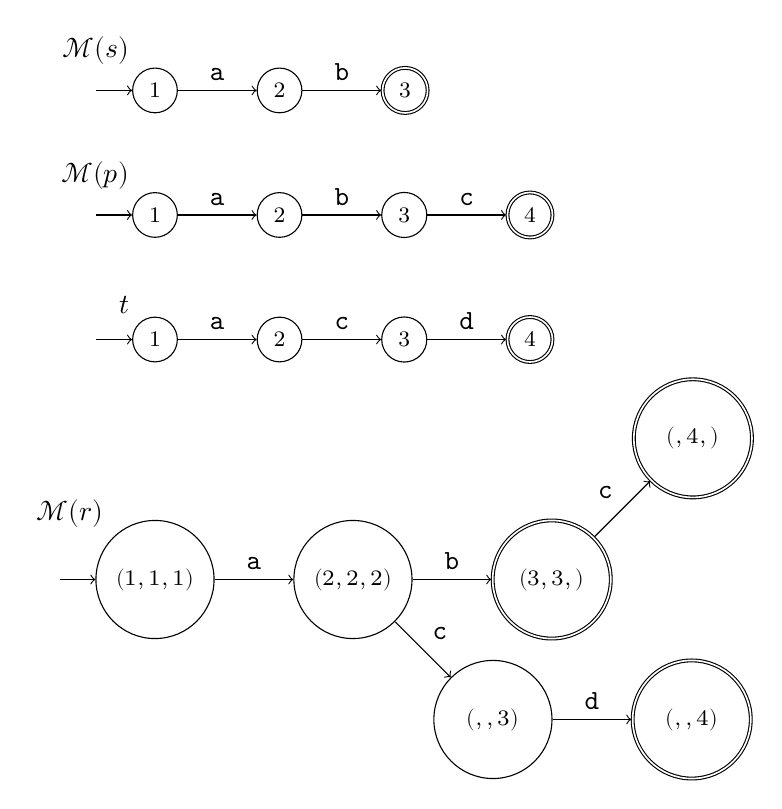
\begin{tikzpicture}
    \tikzset{
      node distance=1cm,
      every state/.append style={minimum size=0.5cm},
      initial text=$ $,
      large/.style={minimum size=1.5cm},
    }

    \node[state, initial, label=above left:$\Automaton{s}$] (x0) {1};
    \node[state, right=of x0] (x1) {2};
    \node[state, accepting, right=of x1] (x2) {3};

    \draw (x0) edge[->] node[auto]{$\Char{a}$} (x1);
    \draw (x1) edge[->] node[auto]{$\Char{b}$} (x2);

    \node[state, initial, label=above left:$\Automaton{p}$, below=of x0] (y0) {1};
    \node[state, right=of y0] (y1) {2};
    \node[state, right=of y1] (y2) {3};
    \node[state, accepting, right=of y2] (y3) {4};

    \draw (y0) edge[->] node[auto]{$\Char{a}$} (y1);
    \draw (y1) edge[->] node[auto]{$\Char{b}$} (y2);
    \draw (y2) edge[->] node[auto]{$\Char{c}$} (y3);

    \node[state, initial, label=above left:$t$, below=of y0] (z0) {1};
    \node[state, right=of z0] (z1) {2};
    \node[state, right=of z1] (z2) {3};
    \node[state, accepting, right=of z2] (z3) {4};

    \draw (z0) edge[->] node[auto]{$\Char{a}$} (z1);
    \draw (z1) edge[->] node[auto]{$\Char{c}$} (z2);
    \draw (z2) edge[->] node[auto]{$\Char{d}$} (z3);

    \node[state, large, initial, below=2cm of z0, label=above left:$\Automaton{r}$] (u0) {$(1,1,1)$};
    \node[state, large, right=of u0] (u1) {$(2, 2, 2)$};
    \node[state, large, accepting, right=of u1] (u2) {$(3,3,\Err)$};
    \draw (u0) edge[->] node[auto]{$\Char{a}$} (u1);
    \draw (u1) edge[->] node[auto]{$\Char{b}$} (u2);

    \node[state, large, accepting, above right=of u2] (u3) {$(\Err, 4, \Err)$};
    \draw (u2) edge[->] node[auto]{$\Char{c}$} (u3);

    \node[state, large, below right=of u1] (u4) {$(\Err,\Err,3)$};
    \node[state, large, accepting, right=of u4] (u5) {$(\Err,\Err,4)$};

    \draw (u1) edge[->] node[auto]{$\Char{c}$} (u4);
    \draw (u4) edge[->] node[auto]{$\Char{d}$} (u5);
  \end{tikzpicture}
\end{center}

Za $(q_1, q_2) \in Q$, če $\acc_1(q_1) \neq \acc_2(q_2)$ potem kot $\acc((q_1, q_2))$ izberemo ali $\acc_1(q_1)$ ali $\acc_2(q_2)$ glede na prioriteto.
Na primer, če združimo avtomata za imena spremenljivk in za ključne besede, vedno izberemo vrednost, ki ustreza avtomatu za ključne besede.
\Next

\subsection*{Primeri}
\subsubsection{Ključne besede}

\begin{align*}
  \N{s} &= \Char{i} \Spc \Char{f} \\
  \N{p} &= \Char{f} \Spc \Char{o} \Spc \Char{r} \\
  \N{t} &= \Char{f} \Spc \Char{o} \Spc \Char{r} \Spc \Char{e} \Spc \Char{a} \Spc \Char{c} \Spc \Char{h} \\
  \N{r} &= \N{s} \Union \N{p} \Union \N{t}
\end{align*}
\Next

\subsection{Opcija}
\Reset

\begin{tcolorbox}[title={Definicija}]
  \begin{equation*}
    \begin{aligned}
      \Opt{s} &= \Null \Union s\\
      \Language{\Opt{s}} &= \{\Str{}\} \cup \Language{s}
    \end{aligned}
  \end{equation*}
\end{tcolorbox}

Ujemanje $s$ 0 ali 1 krat.

Končni avtomat opcije $\Automaton{\Opt{s}}$ lahko sestavimo kot unijo $\Automaton{\Null}$ in $\Automaton{s}$.
Obstaja pa tudi lažji način, $\Automaton{\Opt{s}}$ dobimo tudi, če označimo začetno stanje avtomata $\Automaton{s}$ kot končno.

\begin{center}
  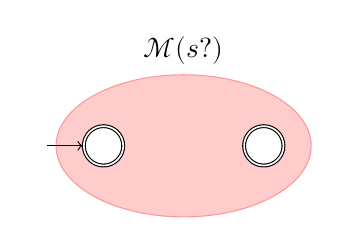
\begin{tikzpicture}
    \tikzset{
      node distance=1cm,
      every state/.append style={fill=white, minimum size=0.5cm},
      initial text=$ $
    }

    %\node[state, initial, accepting] (q0) {};

    \node[state, initial, accepting] (s0) {};
    \node[state, hide, above right=0.15cm and 0.5cm of s0] (s1) {};
    \node[state, hide, below right=0.15cm and 0.5cm of s0] (s2) {};
    \node[state, accepting, right=1.5cm of s0] (sn) {};

    \begin{pgfonlayer}{background}
      \node[fit=(s0) (s1) (s2) (sn), ellip, draw=red!40, fill=red!20, label=above:$\Automaton{\Opt{s}}$] (qm) {};
    \end{pgfonlayer}

  \end{tikzpicture}
\end{center}

\Ex
\begin{center}
  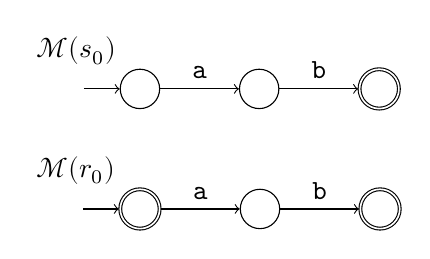
\begin{tikzpicture}
    \tikzset{
      node distance=1cm,
      every state/.append style={minimum size=0.5cm},
      initial text=$ $
    }

    \node[state, initial, label=above left:$\Automaton{\N{s}}$] (x0) {};
    \node[state, right=of x0] (x1) {};
    \node[state, accepting, right=of x1] (x2) {};

    \draw (x0) edge[->] node[auto]{$\Char{a}$} (x1);
    \draw (x1) edge[->] node[auto]{$\Char{b}$} (x2);

    \node[state, initial, accepting, label=above left:$\Automaton{\N{r}}$, below=of x0] (y0) {};
    \node[state, right=of y0] (y1) {};
    \node[state, accepting, right=of y1] (y2) {};

    \draw (y0) edge[->] node[auto]{$\Char{a}$} (y1);
    \draw (y1) edge[->] node[auto]{$\Char{b}$} (y2);
  \end{tikzpicture}
\end{center}

\begin{align*}
  \N{s} &= \Char{a} \Spc \Char{b} \\
  \N{r} &= (\Char{a} \Spc \Char{b})?
\end{align*}

\begin{align*}
  \Language{\N{s}} &= \{\Str{ab}\} \\
  \Language{\N{r}} &= \{\Str{}, \Str{ab}\} \\
\end{align*}

\subsection{Kleene-ovo zaprtje}
\Reset

\begin{tcolorbox}[title={Definicija}]
  \begin{equation*}
    \begin{aligned}
      \Kleene{s} &= \Null \Union s \Union s \Seq s \Union s \Seq s \Seq s \Union \ldots \\
      &= \Rep{s}{0} \Union \Rep{s}{1} \Union \Rep{s}{2} \Union \ldots \\
      &= \Big\vert_{i = 0}^\infty \Rep{s}{i}\\
      \Language{\Kleene{s}} &= \bigcup_{i = 0}^\infty \Language{s^i}
    \end{aligned}
  \end{equation*}
\end{tcolorbox}

Ujemanje $s$ 0 ali več krat.
Z drugimi besedami, $s$ je lahko ponovljen $0, 1, 2, \dots, \infty$ krat.

\begin{tcolorbox}[title={Pravila}]
  \begin{equation*}
    \begin{aligned}
      \Kleene{\Empty} &= \Null\\
      \Kleene{\Null} &= \Null\\
      \Null \Union \Kleene{s} &= \Kleene{s}\\
      \Kleene{s} \Union \Null &= \Kleene{s}\\
      \Kleene{(\Kleene{s})} &= \Kleene{s}\\
      \Kleene{(s \Union t)} &= \Kleene{(\Kleene{s} \Seq t)} \Seq \Kleene{s}\\
      \Kleene{(s \Seq t)} &= \Null \Union s \Seq \Kleene{(t \Seq s)} \Seq t\\
      \Kleene{s} &= (\Null \Union s \Union ... \Union \Rep{s}{i - 1}) \Seq \Kleene{(\Rep{s}{i})}
    \end{aligned}
  \end{equation*}
\end{tcolorbox}

Končni avtomat za Kleeno-ovo zaprtje $\Automaton{\Kleene{s}}$ sestavimo tako:
\begin{enumerate}
  \item Ustvarimo prehod $\delta(q, \Char{a}) = q'$ iz vsakega končnega stanja $q$ v $\Automaton{s}$ v vsako stanje $q'$, ki je direktno dosegljivo iz začetnega stanja istega avtomata.
    Ustvarjen prehod je označen z enakim simbolom $\Char{a}$, kot obstoječi prehod, ki vodi iz začetnega stanja v $q'$.
  \item Začetno stanje označimo kot končno.
\end{enumerate}

\begin{center}
  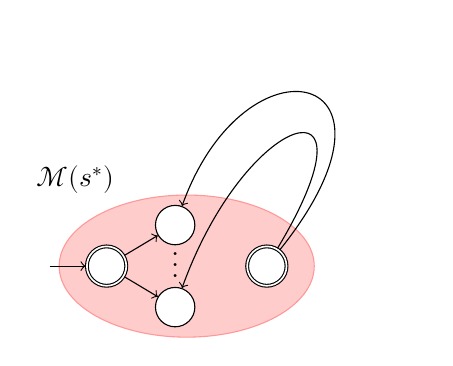
\begin{tikzpicture}
    \tikzset{
      node distance=1cm,
      every state/.append style={fill=white, minimum size=0.5cm},
      initial text=$ $
    }

    \node[state, initial, accepting] (s0) {};
    \node[state, above right=0.15cm and 0.5cm of s0] (s1) {};
    \node[state, below right=0.15cm and 0.5cm of s0] (s2) {};
    \node at ($(s1)!0.5!(s2)$) {\Dots{}};
    \draw (s0) edge[->] (s1);
    \draw (s0) edge[->] (s2);
    \node[state, accepting, right=1.5cm of s0] (sn) {};

    \draw (sn) edge[->, controls={+(2.0,2.5) and +(0.9, 2.5)}] (s1);
    \draw (sn) edge[->, controls={+(1.5,2.5) and +(0.9, 2.5)}] (s2);

    \begin{pgfonlayer}{background}
      \node[fit=(s0) (s1) (s2) (sn), ellip, draw=red!40, fill=red!20, label=above left:$\Automaton{\Kleene{s}}$] (qm) {};
    \end{pgfonlayer}

  \end{tikzpicture}
\end{center}

\Ex
\begin{align*}
  \N{s} &= \Char{a} \\
  \N{r} &= \Kleene{\Char{a}}
\end{align*}

\begin{align*}
  \Language{\N{s}} &= \{\Str{a}\} \\
  \Language{\N{r}} &= \{\Str{}, \Str{a}, \Str{aa}, \Str{aaa}, \dots\} \\
\end{align*}

\begin{center}
  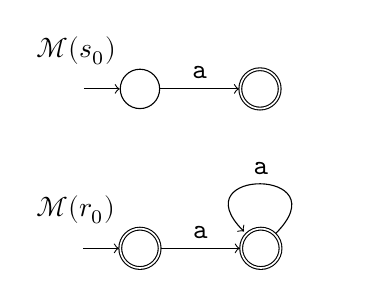
\begin{tikzpicture}
    \tikzset{
      ->,
      node distance=1cm,
      every state/.append style={minimum size=0.5cm},
      initial text=$ $
    }

    \node[state, initial, label=above left:$\Automaton{\N{s}}$] (q0) {};
    \node[state, accepting, right=of q0] (q1) {};

    \draw (q0) edge node[auto]{$\Char{a}$} (q1);

    \node[state, accepting, initial, label=above left:$\Automaton{\N{r}}$, below=1.5cm of q0] (p0) {};
    \node[state, accepting, right=of p0] (p1) {};

    \draw (p0) edge node[auto]{$\Char{a}$} (p1);
    \draw (p1) edge[loop] node[above]{$\Char{a}$} (p1);
  \end{tikzpicture}
\end{center}
\Next

\Ex
\begin{align*}
  \N{s} &= \Char{a} \Spc \Char{b} \\
  \N{r} &= \Kleene{(\Char{a} \Spc \Char{b})}
\end{align*}

\begin{align*}
  \Language{\N{s}} &= \{\Str{ab}\} \\
  \Language{\N{r}} &= \{\Str{}, \Str{ab}, \Str{abab}, \Str{ababab}, \dots\}
\end{align*}

\begin{center}
  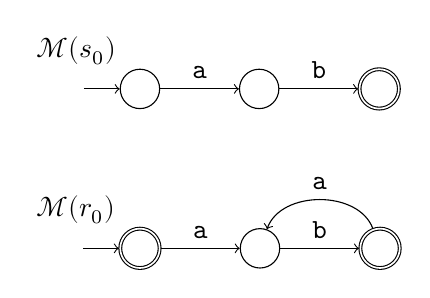
\begin{tikzpicture}
    \tikzset{
      ->,
      node distance=1cm,
      every state/.append style={minimum size=0.5cm},
      initial text=$ $
    }

    \node[state, initial, label=above left:$\Automaton{\N{s}}$] (q0) {};
    \node[state, right=of q0] (q1) {};
    \node[state, accepting, right=of q1] (q2) {};

    \draw (q0) edge node[auto]{$\Char{a}$} (q1);
    \draw (q1) edge node[auto]{$\Char{b}$} (q2);

    \node[state, accepting, label=above left:$\Automaton{\N{r}}$, initial, below=1.5cm of q0] (p0) {};
    \node[state, right=of p0] (p1) {};
    \node[state, accepting, right=of p1] (p2) {};

    \draw (p0) edge node[auto]{$\Char{a}$} (p1);
    \draw (p1) edge node[auto]{$\Char{b}$} (p2);
    \draw (p2) edge[bend right=70] node[above]{$\Char{a}$} (p1);
  \end{tikzpicture}
\end{center}
\Next

\Ex

\begin{align*}
  \N{s} &= \Char{c}\\
  \N{t} &= \Kleene{(\Char{a} \Spc \Char{b})}\\
  \N{r} &= \Char{c} \Seq \Kleene{(\Char{a} \Spc \Char{b})}
\end{align*}

\begin{align*}
  \Language{\N{s}} &= \{\Str{c}\} \\
  \Language{\N{t}} &= \{\Str{}, \Str{ab}, \Str{abab}, \Str{ababab}, \dots\}\\
  \Language{\N{r}} &= \{\Str{c}, \Str{cab}, \Str{cabab}, \Str{cababab}, \dots\}
\end{align*}

\begin{center}
  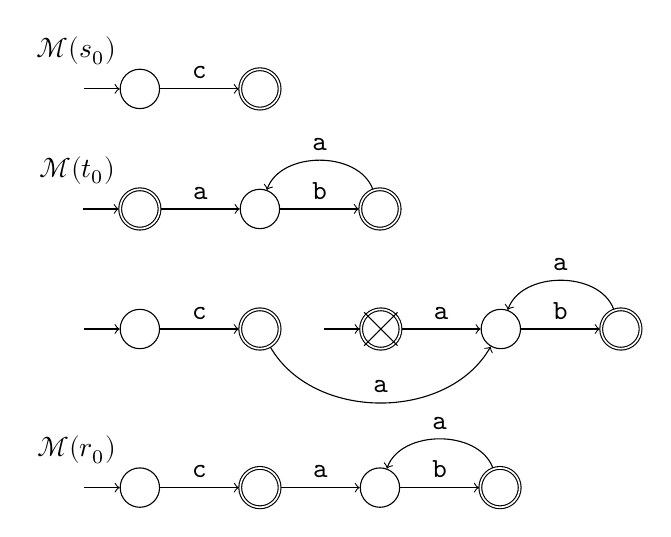
\begin{tikzpicture}
    \tikzset{
      node distance=1cm,
      every state/.append style={minimum size=0.5cm},
      initial text=$ $
    }

    \node[state, initial, label=above left:$\Automaton{\N{s}}$] (x0) {};
    \node[state, accepting, right=of x0] (x1) {};

    \draw (x0) edge[->] node[auto]{$\Char{c}$} (x1);

    \node[state, initial, accepting, label=above left:$\Automaton{\N{t}}$, below=of x0] (y0) {};
    \node[state, right=of y0] (y1) {};
    \node[state, accepting, right=of y1] (y2) {};

    \draw (y0) edge[->] node[auto]{$\Char{a}$} (y1);
    \draw (y1) edge[->] node[auto]{$\Char{b}$} (y2);
    \draw (y2) edge[bend right=70, ->] node[above]{$\Char{a}$} (y1);

    \node[state, initial, below=of y0] (q0) {};
    \node[state, accepting, right=of q0] (q1) {};

    \draw (q0) edge[->] node[auto]{$\Char{c}$} (q1);

    \node[state, initial, accepting, right=of q1] (p0) {};
    \path (p0) pic {cross=0.30cm};
    \node[state, right=of p0] (p1) {};
    \node[state, accepting, right=of p1] (p2) {};

    \draw (p0) edge[->] node[auto]{$\Char{a}$} (p1);
    \draw (p1) edge[->] node[auto]{$\Char{b}$} (p2);

    \draw (q1) edge[->, bend right=60] node[auto]{$\Char{a}$} (p1);
    \draw (p2) edge[bend right=70, ->] node[above]{$\Char{a}$} (p1);

    \node[state, initial, label=above left:$\Automaton{\N{r}}$, below=1.5cm of q0] (s0) {};
    \node[state, accepting, right=of s0] (s1) {};
    \node[state, right=of s1] (s3) {};
    \node[state, accepting, right=of s3] (s4) {};

    \draw (s0) edge[->] node[auto]{$\Char{c}$} (s1);
    \draw (s1) edge[->] node[auto]{$\Char{a}$} (s3);
    \draw (s3) edge[->] node[auto]{$\Char{b}$} (s4);
    \draw (s4) edge[bend right=70, ->] node[above]{$\Char{a}$} (s3);
  \end{tikzpicture}
\end{center}
\Next

\Ex
\begin{align*}
  \N{s} &= \Char{a} \Union \Char{b}\\
  \N{r} &= \Kleene{(\Char{a} \Union \Char{b})}
\end{align*}

\begin{align*}
  \Language{\N{s}} &= \{\Str{a}, \Str{b}\} \\
  \Language{\N{r}} &= \{\Null, \Str{a}, \Str{b}, \Str{aa}, \Str{ab}, \Str{ba}, \Str{bb}, \dots\}\\
\end{align*}

\begin{center}
  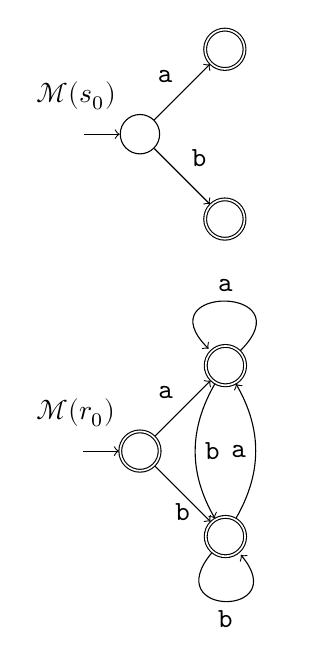
\begin{tikzpicture}
    \tikzset{
      ->,
      node distance=1cm,
      every state/.append style={minimum size=0.5cm},
      initial text=$ $
    }

    \node[state, initial, label=above left:$\Automaton{\N{s}}$] (q0) {};
    \node[state, accepting, above right=of q0] (q1) {};
    \node[state, accepting, below right=of q0] (q2) {};

    \draw (q0) edge node[auto]{$\Char{a}$} (q1);
    \draw (q0) edge node[auto]{$\Char{b}$} (q2);

    \node[state, accepting, label=above left:$\Automaton{\N{r}}$, initial, below=3.5cm of q0] (p0) {};
    \node[state, accepting, above right=of p0] (p1) {};
    \node[state, accepting, below right=of p0] (p2) {};

    \draw (p0) edge node[auto]{$\Char{a}$} (p1);
    \draw (p0) edge node[below]{$\Char{b}$} (p2);
    \draw (p1) edge[bend right] node[auto]{$\Char{b}$} (p2);
    \draw (p2) edge[bend right] node[auto]{$\Char{a}$} (p1);
    \draw (p1) edge[loop] node[above]{$\Char{a}$} (p1);
    \draw (p2) edge[in=-50,out=-130, loop] node[below]{$\Char{b}$} (p2);
  \end{tikzpicture}
\end{center}
\Next

\Ex
\begin{equation*}
\begin{aligned}
  \N{r} &= \Char{a} \Spc \Char{b} \Union \Kleene{\Char{a}}\\
  &= \Char{a} \Spc \Char{b} \Union \Null \Union \Char{a} \Union \Char{a} \Spc \Char{a} \Union \Char{a} \Spc \Char{a} \Spc \Char{a} \Union \dots\\
  &=  \Null \Union \Char{a} \Spc \Char{b} \Union \Char{a} \Union \Char{a} \Spc \Char{a} \Union \Char{a} \Spc \Char{a} \Spc \Char{a} \Union \dots\\
  &= \Null \Union \Char{a} \Seq (\Char{b} \Union \Null \Union \Char{a} \Union \Char{a} \Spc \Char{a} \Union \dots)\\
  &= \Null \Union \Char{a} \Seq (\Char{b} \Union \Kleene{\Char{a}})\\
  &= \Opt{(\Char{a} \Seq (\Char{b} \Union \Kleene{\Char{a}}))}\\
\end{aligned}
\end{equation*}

\begin{center}
  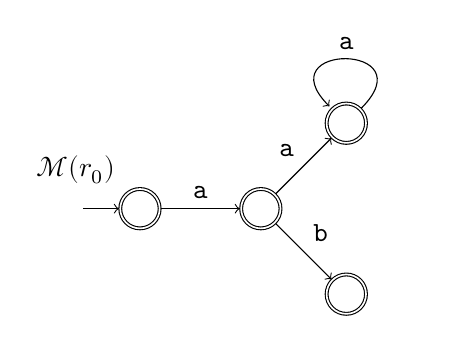
\begin{tikzpicture}
    \tikzset{
      ->,
      node distance=1cm,
      every state/.append style={minimum size=0.5cm},
      initial text=$ $
    }

    \node[state, initial, accepting, label=above left:$\Automaton{\N{r}}$] (i) {};

    \node[state, accepting, right=of i] (q0) {};
    \node[state, accepting, above right=of q0] (q1) {};
    \node[state, accepting, below right=of q0] (q2) {};

    \draw (i) edge node[auto]{$\Char{a}$} (q0);
    \draw (q0) edge node[auto]{$\Char{a}$} (q1);
    \draw (q0) edge node[auto]{$\Char{b}$} (q2);
    \draw (q1) edge[loop] node[above]{$\Char{a}$} (q2);
  \end{tikzpicture}
\end{center}


\subsection{Pozitivno zaprtje}
\Reset

\begin{tcolorbox}[title={Definicija}]
  \begin{equation*}
    \begin{aligned}
      \KleenePlus{s} &= s \Union s \Seq s \Union s \Seq s \Seq s \Union \ldots \\
      &= \Rep{s}{1} \Union \Rep{s}{2} \Union \ldots \\
      &= \Big\vert_{i = 1}^\infty \Rep{s}{i}\\
      \Language{\KleenePlus{s}} &= \bigcup_{i = 1}^\infty \Language{s^i}\\[1em]
      \Kleene{s} &= \Null \Union \KleenePlus{s} = \Opt{(\KleenePlus{s})} = \KleenePlus{(\Opt{s})}\\
      \Language{\Kleene{r}} &= \{\Str{}\} \cup \Language{\KleenePlus{r}}
    \end{aligned}
  \end{equation*}
\end{tcolorbox}

Ujemanje $s$ 1 ali več krat.
Z drugimi besedami, $s$ je lahko ponovljen $1, 2, \dots, \infty$ krat.

Končen avtomat pozitivnega zaprtja sestavimo enako, kot za Kleene-ovo zaprtje, z razliko, da pustimo začetno stanje brez sprememb.
\begin{center}
  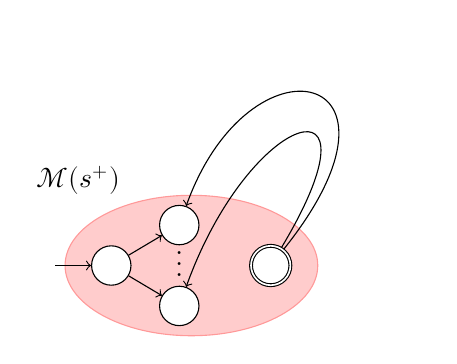
\begin{tikzpicture}
    \tikzset{
      node distance=1cm,
      every state/.append style={fill=white, minimum size=0.5cm},
      initial text=$ $
    }

    \node[state, initial] (s0) {};
    \node[state, above right=0.15cm and 0.5cm of s0] (s1) {};
    \node[state, below right=0.15cm and 0.5cm of s0] (s2) {};
    \node at ($(s1)!0.5!(s2)$) {\Dots{}};
    \draw (s0) edge[->] (s1);
    \draw (s0) edge[->] (s2);
    \node[state, accepting, right=1.5cm of s0] (sn) {};

    \draw (sn) edge[->, controls={+(2.0,2.5) and +(0.9, 2.5)}] (s1);
    \draw (sn) edge[->, controls={+(1.5,2.5) and +(0.9, 2.5)}] (s2);

    \begin{pgfonlayer}{background}
      \node[fit=(s0) (s1) (s2) (sn), ellip, draw=red!40, fill=red!20, label=above left:$\Automaton{\KleenePlus{s}}$] (qm) {};
    \end{pgfonlayer}

  \end{tikzpicture}
\end{center}

\Ex
\begin{align*}
  \N{s} &= \Char{a} \\
  \N{r} &= \KleenePlus{\Char{a}}
\end{align*}

\begin{align*}
  \Language{\N{s}} &= \{\Str{a}\} \\
  \Language{\N{r}} &= \{\Str{a}, \Str{aa}, \Str{aaa}, \dots\} \\
\end{align*}

\begin{center}
  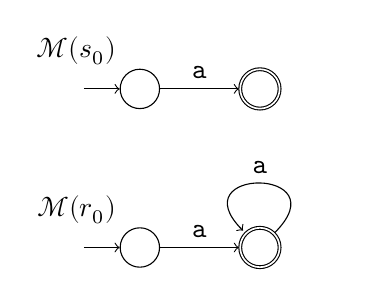
\begin{tikzpicture}
    \tikzset{
      ->,
      node distance=1cm,
      every state/.append style={minimum size=0.5cm},
      initial text=$ $
    }

    \node[state, initial, label=above left:$\Automaton{\N{s}}$] (q0) {};
    \node[state, accepting, right=of q0] (q1) {};

    \draw (q0) edge node[auto]{$\Char{a}$} (q1);

    \node[state, initial, label=above left:$\Automaton{\N{r}}$, below=1.5cm of q0] (p0) {};
    \node[state, accepting, right=of p0] (p1) {};

    \draw (p0) edge node[auto]{$\Char{a}$} (p1);
    \draw (p1) edge[loop] node[above]{$\Char{a}$} (p1);
  \end{tikzpicture}
\end{center}
\Next

\Ex
\begin{align*}
  \N{s} &= \Char{a}? \\
  \N{r} &= \KleenePlus{(\Char{a}?)}
\end{align*}

\begin{align*}
  \Language{\N{s}} &= \{\Str{}, \Str{a}\} \\
  \Language{\N{r}} &= \{\Str{}, \Str{a}, \Str{aa}, \Str{aaa}, \dots\} \\
\end{align*}

\begin{center}
  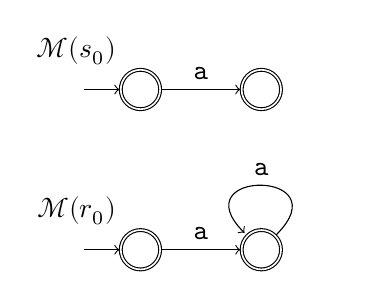
\begin{tikzpicture}
    \tikzset{
      ->,
      node distance=1cm,
      every state/.append style={minimum size=0.5cm},
      initial text=$ $
    }

    \node[state, accepting, initial, label=above left:$\Automaton{\N{s}}$] (q0) {};
    \node[state, accepting, right=of q0] (q1) {};

    \draw (q0) edge node[auto]{$\Char{a}$} (q1);

    \node[state, accepting, initial, label=above left:$\Automaton{\N{r}}$, below=1.5cm of q0] (p0) {};
    \node[state, accepting, right=of p0] (p1) {};

    \draw (p0) edge node[auto]{$\Char{a}$} (p1);
    \draw (p1) edge[loop] node[above]{$\Char{a}$} (p1);
  \end{tikzpicture}
\end{center}
\Next

\subsection*{Primeri}
\subsubsection{Števila}
\begin{align*}
  \N{s} &= \{\Char{0}, \dots, \Char{9}\} \\
  \N{r} &= \KleenePlus{\N{s}}
\end{align*}
\Next

\subsubsection{Naravna števila}
\begin{equation*}
  \Language{\N{r}} = \{\Str{1}, \Str{2}, \dots\}
\end{equation*}
\Next

\subsubsection{Cela števila}
\begin{align*}
  \N{s} &= \{\Char{0}, \dots, \Char{9}\} \\
  \N{r} &= (\Char{+} \Union \Char{-}) \Seq \KleenePlus{\N{s}}
\end{align*}
\Next

\subsubsection{Heksadecimalna števila}
\begin{equation*}
  \Language{\N{r}} = \{\Str{0x0}, \Str{0x1}, \dots, \Str{0xA}, \dots, \Str{0xFFFF}, \dots\}
\end{equation*}
\Next

\subsubsection{Barve}
\begin{equation*}
  \Language{\N{r}} = \{\Str{\#000000}, \dots, \Str{\#FFFFFF}\}
\end{equation*}
\Next

\subsubsection{Števila s plavajočo vejico}
\begin{align*}
  \N{s} &= \{\Char{0}, \dots, \Char{9}\} \\
  \N{r} &= (\Char{+} \Union \Char{-}) \Seq \KleenePlus{\N{s}} \Spc \Char{.} \Spc \Kleene{\N{s}}
\end{align*}
\Next

\subsubsection{Imena spremenljivk}
\begin{align*}
  \N{l} &= \{\Char{a}, \dots, \Char{z}\} \\
  \N{r} &= \KleenePlus{\N{l}}
\end{align*}

\begin{center}
  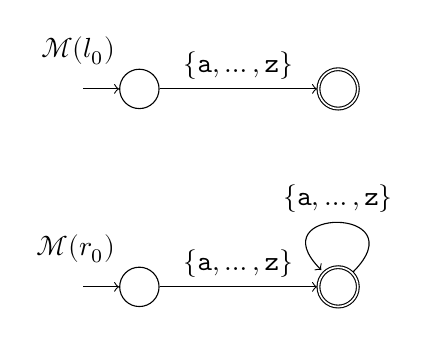
\begin{tikzpicture}
    \tikzset{
      ->,
      node distance=1cm,
      every state/.append style={minimum size=0.5cm},
      initial text=$ $
    }

    \node[state, initial, label=above left:$\Automaton{\N{l}}$] (q0) {};
    \node[state, accepting, right=2cm of q0] (q1) {};

    \draw (q0) edge node[auto]{$\{\Char{a}, \dots, \Char{z}\}$} (q1);

    \node[state, initial, label=above left:$\Automaton{\N{r}}$, below=2.0cm of q0] (p0) {};
    \node[state, accepting, right=2cm of p0] (p1) {};

    \draw (p0) edge node[auto]{$\{\Char{a}, \dots, \Char{z}\}$} (p1);
    \draw (p1) edge[loop] node[above]{$\{\Char{a}, \dots, \Char{z}\}$} (p1);
  \end{tikzpicture}
\end{center}
\Next

\subsubsection{Ključne besede in imena spremenljivk}
\begin{align*}
  \N{i} &= \KleenePlus{\{\Char{a}, \dots, \Char{z}\}}\\
  \N{k} &= \Char{a} \Spc \Char{b} \Union \Char{a} \Spc \Char{b} \Spc \Char{c} \Union \Char{a} \Spc \Char{c} \Spc \Char{d}\\
  \N{r} &= \N{i} \Union \N{k}
\end{align*}

\begin{equation*}
  A = \{\Char{a}, \dots, \Char{z}\}
\end{equation*}

Gre tudi z izpostavljanjem, vendar je nastali regularni izraz precej kompleksen.
\begin{equation*}
\begin{aligned}
  \N{r} &= \Char{a} \Spc \Char{b} \Union \Char{a} \Spc \Char{b} \Spc \Char{c} \Union \Char{a} \Spc \Char{c} \Spc \Char{d} \Union \KleenePlus{A}\\
  &= \underline{\Char{a}} \Seq (\Char{b} \Union \Char{b} \Spc \Char{c} \Union \Char{c} \Spc \Char{d} \Union \Kleene{A}) \Union (A - \{\Char{a}\}) \Seq \Kleene{A}\\ 
  &= \Char{a} \Seq (\Null \Union \underline{\Char{b}} \Seq (\not\Null \Union \Char{c} \Union \Kleene{A}) \Union \underline{\Char{c}} \Seq (\Char{d} \Union \Kleene{A}) \Union (A - \{\Char{b}, \Char{c}\}) \Seq \Kleene{A}) \Union (A - \{\Char{a}\}) \Seq \Kleene{A} \\
  &= \Char{a} \Seq (\Null \Union \Char{b} \Seq (\Char{c} \Union \Kleene{A}) \Union \Char{c} \Seq (\Char{d} \Union \Kleene{A}) \Union (A - \{\Char{b}, \Char{c}\}) \Seq \Kleene{A}) \Union (A - \{\Char{a}\}) \Seq \Kleene{A}\\
  &= \Char{a} \Seq (\Null \Union \Char{b} \Seq (\Null \Union \underline{\Char{c}} \Seq (\not\Null \Union \Kleene{A}) \Union (A - \{\Char{c}\}) \Seq \Kleene{A}) \Union \Char{c} \Seq (\Char{d} \Union \Kleene{A}) \Union (A - \{\Char{b}, \Char{c}\}) \Seq \Kleene{A}) \Union (A - \{\Char{a}\}) \Seq \Kleene{A}\\
  &= \Char{a} \Seq (\Null \Union \Char{b} \Seq (\Null \Union \Char{c} \Seq \Kleene{A} \Union (A - \{\Char{c}\}) \Seq \Kleene{A}) \Union \Char{c} \Seq (\Char{d} \Union \Kleene{A}) \Union (A - \{\Char{b}, \Char{c}\}) \Seq \Kleene{A}) \Union (A - \{\Char{a}\}) \Seq \Kleene{A}\\
  &= \Char{a} \Seq (\Null \Union \Char{b} \Seq (\Null \Union \Char{c} \Seq \Kleene{A} \Union (A - \{\Char{c}\}) \Seq \Kleene{A}) \Union \Char{c} \Seq (\Null \Union \underline{\Char{d}} \Seq (\not\Null \Union \Kleene{A}) \Union (A - \{\Char{d}\}) \Seq \Kleene{A}) \Union (A - \{\Char{b}, \Char{c}\}) \Seq \Kleene{A}) \Union (A - \{\Char{a}\}) \Seq \Kleene{A}\\
  &= \Char{a} \Seq (\Null \Union \Char{b} \Seq (\Null \Union \Char{c} \Seq \Kleene{A} \Union (A - \{\Char{c}\}) \Seq \Kleene{A}) \Union \Char{c} \Seq (\Null \Union \Char{d} \Seq \Kleene{A} \Union (A - \{\Char{d}\}) \Seq \Kleene{A}) \Union (A - \{\Char{b}, \Char{c}\}) \Seq \Kleene{A}) \Union (A - \{\Char{a}\}) \Seq \Kleene{A}\\
\end{aligned}
\end{equation*}

Zato raje uporabimo konstrukcijo kartezičnega produkta.
\begin{align*}
  \acc_{\N{i}}(2) &= 1 \\[1em]
  \acc_{\N{k}}(3) &= 2 \\
  \acc_{\N{k}}(4) &= 2 \\
  \acc_{\N{k}}(6) &= 2 \\
\end{align*}

\begin{center}
  \begin{tikzpicture}
    \tikzset{
      ->,
      node distance=1cm,
      every state/.append style={minimum size=0.5cm},
      initial text=$ $
    }

    \node[state, initial, label=above left:$\Automaton{\N{i}}$, below=2.0cm of q0] (p0) {1};
    \node[state, accepting, right=2cm of p0] (p1) {2};

    \draw (p0) edge node[auto]{$\{\Char{a}, \dots, \Char{z}\}$} (p1);
    \draw (p1) edge[loop] node[above]{$\{\Char{a}, \dots, \Char{z}\}$} (p1);

    \node[state, initial, label=above left:$\Automaton{\N{k}}$, below=1.5cm of p0] (u0) {1};
    \node[state, right=of u0] (u1) {2};
    \node[state, accepting, right=of u1] (u2) {3};
    \draw (u0) edge[->] node[auto]{$\Char{a}$} (u1);
    \draw (u1) edge[->] node[auto]{$\Char{b}$} (u2);

    \node[state, accepting, right=of u2] (u3) {4};
    \draw (u2) edge[->] node[auto]{$\Char{c}$} (u3);

    \node[state, below right=of u1] (u4) {5};
    \node[state, accepting, right=of u4] (u5) {6};

    \draw (u1) edge[->] node[auto]{$\Char{c}$} (u4);
    \draw (u4) edge[->] node[auto]{$\Char{d}$} (u5);
  \end{tikzpicture}
\end{center}

\begin{center}
  \begin{tikzpicture}
    \tikzset{
      ->,
      node distance=1cm,
      every state/.append style={minimum size=0.5cm},
      large/.style={minimum size=1.2cm},
      initial text=$ $
    }

    \node[state, large, initial, label=above left:$\Automaton{\N{r}}$] (v0) {$(1,1)$};
    \node[state, large, accepting, right=of v0] (v1) {(2,2)};
    \node[state, large, accepting, right=of v1] (v2) {$(2, 3)$};
    \draw (v0) edge[->] node[auto]{$\Char{a}$} (v1);
    \draw (v1) edge[->] node[auto]{$\Char{b}$} (v2);

    \node[state, large, accepting, right=of v2] (v3) {$(2, 4)$};
    \draw (v2) edge[->] node[auto]{$\Char{c}$} (v3);

    \node[state, large, accepting, below right=of v1] (v4) {$(2, 5)$};
    \node[state, large, accepting, right=of v4] (v5) {$(2, 6)$};

    \draw (v1) edge[->] node[auto]{$\Char{c}$} (v4);
    \draw (v4) edge[->] node[auto]{$\Char{d}$} (v5);

    \node[state, large, accepting, above=2cm of v1] (s) {$(2, \Err)$};
    \draw (v0) edge[->, bend left] node[auto]{$A - \{\Char{a}\}$} (s);
    \draw (v1) edge[->, bend right] node[auto]{$A - \{\Char{b}, \Char{c}\}$} (s);
    \draw (v2) edge[->, bend right] node[right]{$A - \{\Char{c}\}$} (s);
    \draw (v3) edge[->, bend right=50] node[above right]{$A$} (s);
    \draw (v4) edge[->, out=-150, in=170, looseness=3] node[left ]{$A - \{\Char{d}\}$} (s);
    \draw (v5) edge[->, out=0, in=45, looseness=2] node[right]{$A$} (s);
    \draw (s) edge[->, loop] node[above]{$A$} (s);
  \end{tikzpicture}
\end{center}
\begin{align*}
  \acc_{\N{r}}((2, \Err)) &= 1 \\
  \acc_{\N{r}}((2, 2)) &= 1 \\
  \acc_{\N{r}}((2, 3)) &= 2 \\
  \acc_{\N{r}}((2, 4)) &= 2 \\
  \acc_{\N{r}}((2, 5)) &= 1 \\
  \acc_{\N{r}}((2, 6)) &= 2 \\
\end{align*}

\Special{Poseben primer:} Potrebno je samo eno dodatno stanje $(2, \Err)$, v primerjavi z avtomatom za ključne besede.
Stanje $(2, \Err)$ deluje kot ponor.
Množice znakov $A - D$ lahko implementiramo tako, da najprej naredimo vse prehode za A in jih potem "povozimo" s prehodi za D.
\Next

%\section{Dodatno: Konstrukcija podmnožic}
%Pri vajah se bomo omejili na deterministične avtomate.
%Kljub temu pa je pravkar opisana konstrukcija dovolj splošna, da omogoča sestavo avtomatov za vse možne regularne izraze.
%Težava je le, da operatorji ne zagotavljajo, da bo nastali avtomat determinističen.
%Nedeterminističen avtomat lahko pretvorimo v determinističnega z uporabo konstrukcije podmnožic (stanja nastalega avtomata bodo označena s podmnožicami $Q$). 
%
%\begin{algorithm}
%  input: $(Q, \Sigma, \delta, q_{0}, F)$
%  output: $(Q', \Sigma, \delta', q'_{0}, F')$
%  $q'_0$ $\gets$ $\{q_{0}\}$
%
%  $Q'$ $\gets$ $\{q'_0\}$
%  $\delta'$ $\gets$ $\emptyset$
%  foreach $q' \in Q'$
%    foreach $q \in q'$
%      $q''$ $\gets$ $\emptyset$
%      foreach $a \in \Sigma$
%        $q''$ $\gets$ $q'' \cup \{\delta(q, a)\}$
%      $Q'$ $\gets$ $Q' \cup \{q'\}$
%      $\delta'$ $\gets$ $\delta' \cup \{(q', a) \mapsto q''\}$
%  $F'$ $\gets$ $\{q' \mid q' \in Q' \land q' \cap F \neq \emptyset \}$
%\end{algorithm}

\printbibliography
\end{document}
